% !TEX encoding = UTF-8 Unicode
\documentclass[10pt]{standalone}\usepackage{tikz,graphicx}
\usepackage{fontspec}
\setmainfont{Arial}
\setsansfont{Arial}\begin{document}

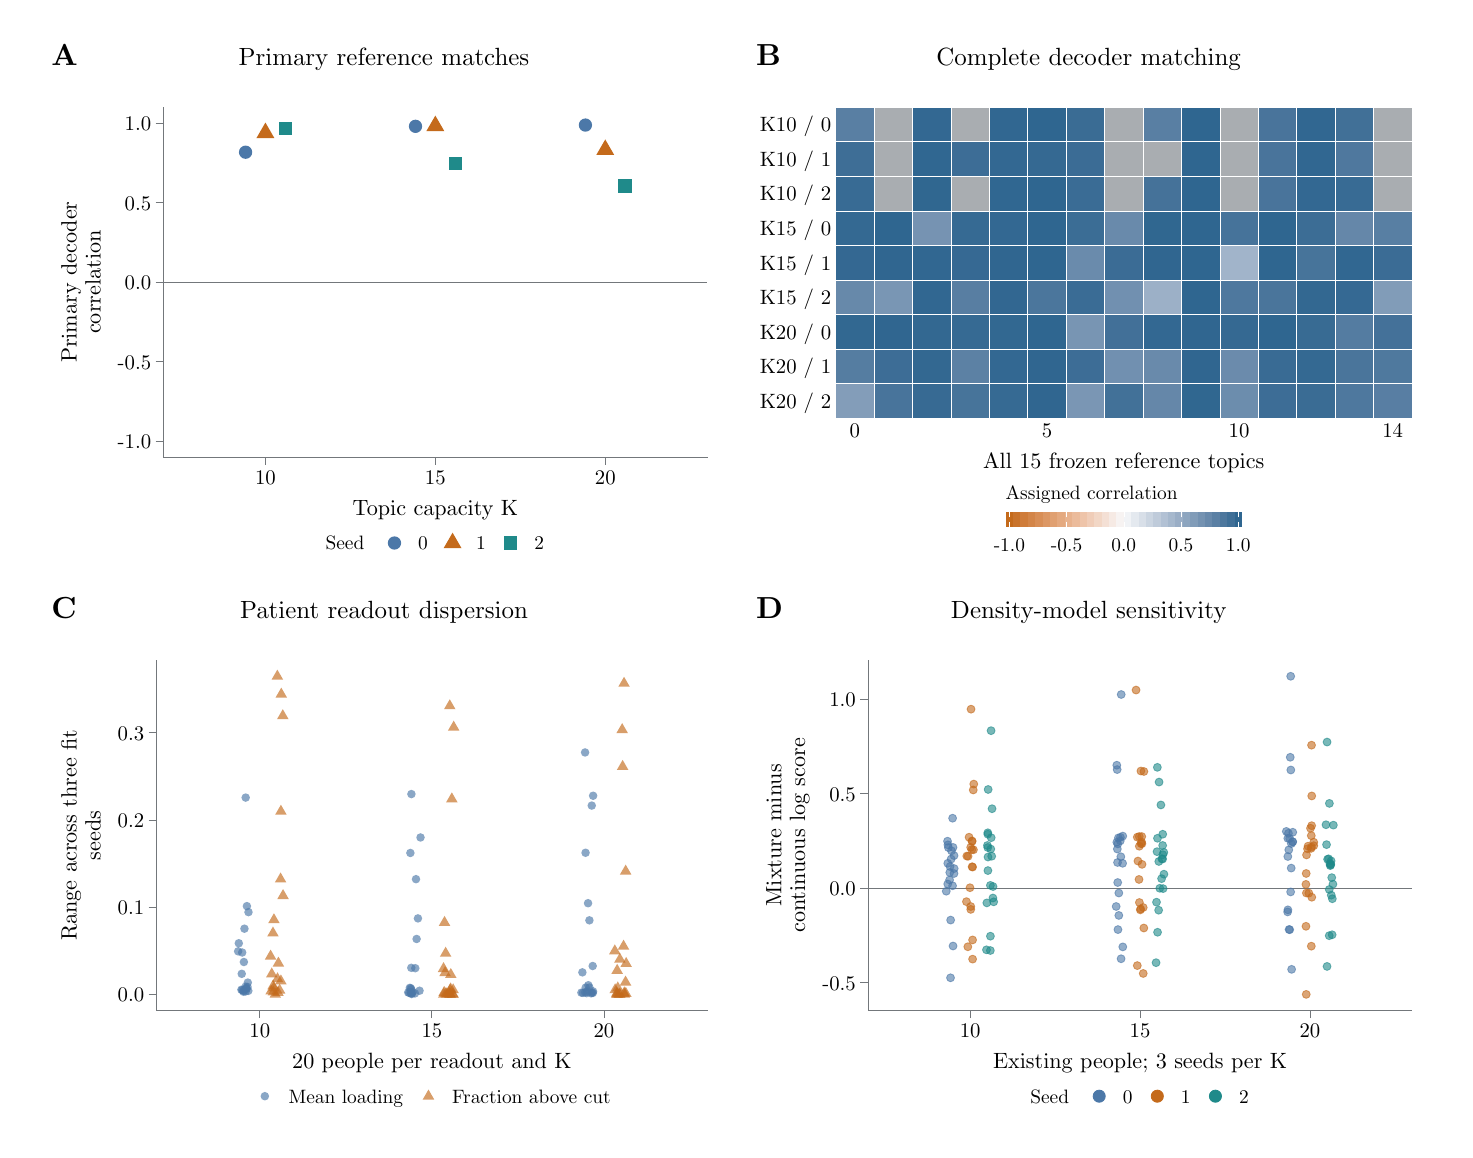
\begin{tikzpicture}[x=1pt,y=1pt]
\definecolor{fillColor}{RGB}{255,255,255}
\path[use as bounding box,fill=fillColor,fill opacity=0.00] (0,0) rectangle (512.15,398.34);
\begin{scope}
\path[clip] (  0.00,  0.00) rectangle (512.15,398.34);
\definecolor{drawColor}{RGB}{0,0,0}

\node[text=drawColor,anchor=base west,inner sep=0pt, outer sep=0pt, scale=  1.10] at (  8.54,384.77) {\bfseries A};

\node[text=drawColor,anchor=base,inner sep=0pt, outer sep=0pt, scale=  0.90] at (128.75,384.78) {Primary reference matches};
\end{scope}
\begin{scope}
\path[clip] (  8.54,204.15) rectangle (248.96,374.72);
\definecolor{fillColor}{RGB}{255,255,255}

\path[fill=fillColor] (  8.54,204.15) rectangle (248.96,374.72);
\end{scope}
\begin{scope}
\path[clip] ( 49.07,243.15) rectangle (245.55,369.60);
\definecolor{fillColor}{RGB}{255,255,255}

\path[fill=fillColor] ( 49.07,243.15) rectangle (245.55,369.60);
\definecolor{drawColor}{RGB}{115,119,123}

\path[draw=drawColor,line width= 0.3pt,line join=round] ( 49.07,306.38) -- (245.55,306.38);
\definecolor{fillColor}{RGB}{76,120,168}

\path[fill=fillColor] ( 78.74,353.33) circle (  2.40);
\definecolor{fillColor}{RGB}{196,106,27}

\path[fill=fillColor] ( 85.91,364.05) --
	( 89.14,358.45) --
	( 82.67,358.45) --
	cycle;
\definecolor{fillColor}{RGB}{31,138,138}

\path[fill=fillColor] ( 90.67,359.45) --
	( 95.47,359.45) --
	( 95.47,364.25) --
	( 90.67,364.25) --
	cycle;
\definecolor{fillColor}{RGB}{76,120,168}

\path[fill=fillColor] (140.14,362.69) circle (  2.40);
\definecolor{fillColor}{RGB}{196,106,27}

\path[fill=fillColor] (147.31,366.57) --
	(150.54,360.97) --
	(144.07,360.97) --
	cycle;
\definecolor{fillColor}{RGB}{31,138,138}

\path[fill=fillColor] (152.07,346.85) --
	(156.87,346.85) --
	(156.87,351.65) --
	(152.07,351.65) --
	cycle;
\definecolor{fillColor}{RGB}{76,120,168}

\path[fill=fillColor] (201.54,363.14) circle (  2.40);
\definecolor{fillColor}{RGB}{196,106,27}

\path[fill=fillColor] (208.71,357.95) --
	(211.94,352.35) --
	(205.47,352.35) --
	cycle;
\definecolor{fillColor}{RGB}{31,138,138}

\path[fill=fillColor] (213.47,338.68) --
	(218.27,338.68) --
	(218.27,343.48) --
	(213.47,343.48) --
	cycle;
\end{scope}
\begin{scope}
\path[clip] (  0.00,  0.00) rectangle (512.15,398.34);
\definecolor{drawColor}{RGB}{115,119,123}

\path[draw=drawColor,line width= 0.3pt,line join=round,line cap=rect] ( 49.07,243.15) --
	( 49.07,369.60);
\end{scope}
\begin{scope}
\path[clip] (  0.00,  0.00) rectangle (512.15,398.34);
\definecolor{drawColor}{RGB}{0,0,0}

\node[text=drawColor,anchor=base east,inner sep=0pt, outer sep=0pt, scale=  0.75] at ( 44.62,246.22) {-1.0};

\node[text=drawColor,anchor=base east,inner sep=0pt, outer sep=0pt, scale=  0.75] at ( 44.62,274.95) {-0.5};

\node[text=drawColor,anchor=base east,inner sep=0pt, outer sep=0pt, scale=  0.75] at ( 44.62,303.69) {0.0};

\node[text=drawColor,anchor=base east,inner sep=0pt, outer sep=0pt, scale=  0.75] at ( 44.62,332.43) {0.5};

\node[text=drawColor,anchor=base east,inner sep=0pt, outer sep=0pt, scale=  0.75] at ( 44.62,361.17) {1.0};
\end{scope}
\begin{scope}
\path[clip] (  0.00,  0.00) rectangle (512.15,398.34);
\definecolor{drawColor}{RGB}{115,119,123}

\path[draw=drawColor,line width= 0.3pt,line join=round] ( 46.22,248.90) --
	( 49.07,248.90);

\path[draw=drawColor,line width= 0.3pt,line join=round] ( 46.22,277.64) --
	( 49.07,277.64);

\path[draw=drawColor,line width= 0.3pt,line join=round] ( 46.22,306.38) --
	( 49.07,306.38);

\path[draw=drawColor,line width= 0.3pt,line join=round] ( 46.22,335.12) --
	( 49.07,335.12);

\path[draw=drawColor,line width= 0.3pt,line join=round] ( 46.22,363.85) --
	( 49.07,363.85);
\end{scope}
\begin{scope}
\path[clip] (  0.00,  0.00) rectangle (512.15,398.34);
\definecolor{drawColor}{RGB}{115,119,123}

\path[draw=drawColor,line width= 0.3pt,line join=round,line cap=rect] ( 49.07,243.15) --
	(245.55,243.15);
\end{scope}
\begin{scope}
\path[clip] (  0.00,  0.00) rectangle (512.15,398.34);
\definecolor{drawColor}{RGB}{115,119,123}

\path[draw=drawColor,line width= 0.3pt,line join=round] ( 85.91,240.31) --
	( 85.91,243.15);

\path[draw=drawColor,line width= 0.3pt,line join=round] (147.31,240.31) --
	(147.31,243.15);

\path[draw=drawColor,line width= 0.3pt,line join=round] (208.71,240.31) --
	(208.71,243.15);
\end{scope}
\begin{scope}
\path[clip] (  0.00,  0.00) rectangle (512.15,398.34);
\definecolor{drawColor}{RGB}{0,0,0}

\node[text=drawColor,anchor=base,inner sep=0pt, outer sep=0pt, scale=  0.75] at ( 85.91,233.34) {10};

\node[text=drawColor,anchor=base,inner sep=0pt, outer sep=0pt, scale=  0.75] at (147.31,233.34) {15};

\node[text=drawColor,anchor=base,inner sep=0pt, outer sep=0pt, scale=  0.75] at (208.71,233.34) {20};
\end{scope}
\begin{scope}
\path[clip] (  0.00,  0.00) rectangle (512.15,398.34);
\definecolor{drawColor}{RGB}{0,0,0}

\node[text=drawColor,anchor=base,inner sep=0pt, outer sep=0pt, scale=  0.80] at (147.31,222.05) {Topic capacity K};
\end{scope}
\begin{scope}
\path[clip] (  0.00,  0.00) rectangle (512.15,398.34);
\definecolor{drawColor}{RGB}{0,0,0}

\node[text=drawColor,rotate= 90.00,anchor=base,inner sep=0pt, outer sep=0pt, scale=  0.80] at ( 17.68,306.38) {Primary decoder};

\node[text=drawColor,rotate= 90.00,anchor=base,inner sep=0pt, outer sep=0pt, scale=  0.80] at ( 26.32,306.38) {correlation};
\end{scope}
\begin{scope}
\path[clip] (  0.00,  0.00) rectangle (512.15,398.34);
\definecolor{fillColor}{RGB}{255,255,255}

\path[fill=fillColor] (107.64,207.56) rectangle (186.98,216.67);
\end{scope}
\begin{scope}
\path[clip] (  0.00,  0.00) rectangle (512.15,398.34);
\definecolor{drawColor}{RGB}{0,0,0}

\node[text=drawColor,anchor=base west,inner sep=0pt, outer sep=0pt, scale=  0.70] at (107.64,209.61) {Seed};
\end{scope}
\begin{scope}
\path[clip] (  0.00,  0.00) rectangle (512.15,398.34);
\definecolor{fillColor}{RGB}{255,255,255}

\path[fill=fillColor] (127.98,207.56) rectangle (137.09,216.67);
\definecolor{fillColor}{RGB}{76,120,168}

\path[fill=fillColor] (132.54,212.12) circle (  2.40);
\end{scope}
\begin{scope}
\path[clip] (  0.00,  0.00) rectangle (512.15,398.34);
\definecolor{fillColor}{RGB}{255,255,255}

\path[fill=fillColor] (148.98,207.56) rectangle (158.09,216.67);
\definecolor{fillColor}{RGB}{196,106,27}

\path[fill=fillColor] (153.54,215.85) --
	(156.77,210.25) --
	(150.30,210.25) --
	cycle;
\end{scope}
\begin{scope}
\path[clip] (  0.00,  0.00) rectangle (512.15,398.34);
\definecolor{fillColor}{RGB}{255,255,255}

\path[fill=fillColor] (169.98,207.56) rectangle (179.09,216.67);
\definecolor{fillColor}{RGB}{31,138,138}

\path[fill=fillColor] (172.13,209.71) --
	(176.93,209.71) --
	(176.93,214.52) --
	(172.13,214.52) --
	cycle;
\end{scope}
\begin{scope}
\path[clip] (  0.00,  0.00) rectangle (512.15,398.34);
\definecolor{drawColor}{RGB}{0,0,0}

\node[text=drawColor,anchor=base west,inner sep=0pt, outer sep=0pt, scale=  0.70] at (141.09,209.61) {0};
\end{scope}
\begin{scope}
\path[clip] (  0.00,  0.00) rectangle (512.15,398.34);
\definecolor{drawColor}{RGB}{0,0,0}

\node[text=drawColor,anchor=base west,inner sep=0pt, outer sep=0pt, scale=  0.70] at (162.09,209.61) {1};
\end{scope}
\begin{scope}
\path[clip] (  0.00,  0.00) rectangle (512.15,398.34);
\definecolor{drawColor}{RGB}{0,0,0}

\node[text=drawColor,anchor=base west,inner sep=0pt, outer sep=0pt, scale=  0.70] at (183.09,209.61) {2};
\end{scope}
\begin{scope}
\path[clip] (  0.00,  0.00) rectangle (512.15,398.34);
\definecolor{drawColor}{RGB}{0,0,0}

\node[text=drawColor,anchor=base west,inner sep=0pt, outer sep=0pt, scale=  1.10] at (263.19,384.77) {\bfseries B};

\node[text=drawColor,anchor=base,inner sep=0pt, outer sep=0pt, scale=  0.90] at (383.40,384.78) {Complete decoder matching};
\end{scope}
\begin{scope}
\path[clip] (263.19,204.15) rectangle (503.61,374.72);
\definecolor{fillColor}{RGB}{255,255,255}

\path[fill=fillColor] (263.19,204.15) rectangle (503.61,374.72);
\end{scope}
\begin{scope}
\path[clip] (291.97,257.29) rectangle (500.20,369.60);
\definecolor{fillColor}{RGB}{255,255,255}

\path[fill=fillColor] (291.97,257.29) rectangle (500.20,369.60);
\definecolor{drawColor}{RGB}{255,255,255}
\definecolor{fillColor}{RGB}{89,127,163}

\path[draw=drawColor,line width= 0.2pt,fill=fillColor] (291.97,357.12) rectangle (305.85,369.60);
\definecolor{fillColor}{RGB}{169,173,177}

\path[draw=drawColor,line width= 0.2pt,fill=fillColor] (305.85,357.12) rectangle (319.73,369.60);
\definecolor{fillColor}{RGB}{51,104,146}

\path[draw=drawColor,line width= 0.2pt,fill=fillColor] (319.73,357.12) rectangle (333.62,369.60);
\definecolor{fillColor}{RGB}{169,173,177}

\path[draw=drawColor,line width= 0.2pt,fill=fillColor] (333.62,357.12) rectangle (347.50,369.60);
\definecolor{fillColor}{RGB}{49,103,145}

\path[draw=drawColor,line width= 0.2pt,fill=fillColor] (347.50,357.12) rectangle (361.38,369.60);
\definecolor{fillColor}{RGB}{47,102,144}

\path[draw=drawColor,line width= 0.2pt,fill=fillColor] (361.38,357.12) rectangle (375.26,369.60);
\definecolor{fillColor}{RGB}{58,108,148}

\path[draw=drawColor,line width= 0.2pt,fill=fillColor] (375.26,357.12) rectangle (389.14,369.60);
\definecolor{fillColor}{RGB}{169,173,177}

\path[draw=drawColor,line width= 0.2pt,fill=fillColor] (389.14,357.12) rectangle (403.03,369.60);
\definecolor{fillColor}{RGB}{89,127,163}

\path[draw=drawColor,line width= 0.2pt,fill=fillColor] (403.03,357.12) rectangle (416.91,369.60);
\definecolor{fillColor}{RGB}{47,102,144}

\path[draw=drawColor,line width= 0.2pt,fill=fillColor] (416.91,357.12) rectangle (430.79,369.60);
\definecolor{fillColor}{RGB}{169,173,177}

\path[draw=drawColor,line width= 0.2pt,fill=fillColor] (430.79,357.12) rectangle (444.67,369.60);
\definecolor{fillColor}{RGB}{73,116,155}

\path[draw=drawColor,line width= 0.2pt,fill=fillColor] (444.67,357.12) rectangle (458.55,369.60);
\definecolor{fillColor}{RGB}{49,103,145}

\path[draw=drawColor,line width= 0.2pt,fill=fillColor] (458.55,357.12) rectangle (472.44,369.60);
\definecolor{fillColor}{RGB}{65,112,151}

\path[draw=drawColor,line width= 0.2pt,fill=fillColor] (472.44,357.12) rectangle (486.32,369.60);
\definecolor{fillColor}{RGB}{169,173,177}

\path[draw=drawColor,line width= 0.2pt,fill=fillColor] (486.32,357.12) rectangle (500.20,369.60);
\definecolor{fillColor}{RGB}{62,110,150}

\path[draw=drawColor,line width= 0.2pt,fill=fillColor] (291.97,344.64) rectangle (305.85,357.12);
\definecolor{fillColor}{RGB}{169,173,177}

\path[draw=drawColor,line width= 0.2pt,fill=fillColor] (305.85,344.64) rectangle (319.73,357.12);
\definecolor{fillColor}{RGB}{48,103,145}

\path[draw=drawColor,line width= 0.2pt,fill=fillColor] (319.73,344.64) rectangle (333.62,357.12);
\definecolor{fillColor}{RGB}{61,109,150}

\path[draw=drawColor,line width= 0.2pt,fill=fillColor] (333.62,344.64) rectangle (347.50,357.12);
\definecolor{fillColor}{RGB}{51,104,146}

\path[draw=drawColor,line width= 0.2pt,fill=fillColor] (347.50,344.64) rectangle (361.38,357.12);
\definecolor{fillColor}{RGB}{53,105,146}

\path[draw=drawColor,line width= 0.2pt,fill=fillColor] (361.38,344.64) rectangle (375.26,357.12);
\definecolor{fillColor}{RGB}{59,108,149}

\path[draw=drawColor,line width= 0.2pt,fill=fillColor] (375.26,344.64) rectangle (389.14,357.12);
\definecolor{fillColor}{RGB}{169,173,177}

\path[draw=drawColor,line width= 0.2pt,fill=fillColor] (389.14,344.64) rectangle (403.03,357.12);

\path[draw=drawColor,line width= 0.2pt,fill=fillColor] (403.03,344.64) rectangle (416.91,357.12);
\definecolor{fillColor}{RGB}{47,102,144}

\path[draw=drawColor,line width= 0.2pt,fill=fillColor] (416.91,344.64) rectangle (430.79,357.12);
\definecolor{fillColor}{RGB}{169,173,177}

\path[draw=drawColor,line width= 0.2pt,fill=fillColor] (430.79,344.64) rectangle (444.67,357.12);
\definecolor{fillColor}{RGB}{73,116,155}

\path[draw=drawColor,line width= 0.2pt,fill=fillColor] (444.67,344.64) rectangle (458.55,357.12);
\definecolor{fillColor}{RGB}{49,103,145}

\path[draw=drawColor,line width= 0.2pt,fill=fillColor] (458.55,344.64) rectangle (472.44,357.12);
\definecolor{fillColor}{RGB}{79,120,158}

\path[draw=drawColor,line width= 0.2pt,fill=fillColor] (472.44,344.64) rectangle (486.32,357.12);
\definecolor{fillColor}{RGB}{169,173,177}

\path[draw=drawColor,line width= 0.2pt,fill=fillColor] (486.32,344.64) rectangle (500.20,357.12);
\definecolor{fillColor}{RGB}{56,107,148}

\path[draw=drawColor,line width= 0.2pt,fill=fillColor] (291.97,332.16) rectangle (305.85,344.64);
\definecolor{fillColor}{RGB}{169,173,177}

\path[draw=drawColor,line width= 0.2pt,fill=fillColor] (305.85,332.16) rectangle (319.73,344.64);
\definecolor{fillColor}{RGB}{48,103,144}

\path[draw=drawColor,line width= 0.2pt,fill=fillColor] (319.73,332.16) rectangle (333.62,344.64);
\definecolor{fillColor}{RGB}{169,173,177}

\path[draw=drawColor,line width= 0.2pt,fill=fillColor] (333.62,332.16) rectangle (347.50,344.64);
\definecolor{fillColor}{RGB}{48,103,145}

\path[draw=drawColor,line width= 0.2pt,fill=fillColor] (347.50,332.16) rectangle (361.38,344.64);
\definecolor{fillColor}{RGB}{47,102,144}

\path[draw=drawColor,line width= 0.2pt,fill=fillColor] (361.38,332.16) rectangle (375.26,344.64);
\definecolor{fillColor}{RGB}{58,108,149}

\path[draw=drawColor,line width= 0.2pt,fill=fillColor] (375.26,332.16) rectangle (389.14,344.64);
\definecolor{fillColor}{RGB}{169,173,177}

\path[draw=drawColor,line width= 0.2pt,fill=fillColor] (389.14,332.16) rectangle (403.03,344.64);
\definecolor{fillColor}{RGB}{69,114,153}

\path[draw=drawColor,line width= 0.2pt,fill=fillColor] (403.03,332.16) rectangle (416.91,344.64);
\definecolor{fillColor}{RGB}{47,102,144}

\path[draw=drawColor,line width= 0.2pt,fill=fillColor] (416.91,332.16) rectangle (430.79,344.64);
\definecolor{fillColor}{RGB}{169,173,177}

\path[draw=drawColor,line width= 0.2pt,fill=fillColor] (430.79,332.16) rectangle (444.67,344.64);
\definecolor{fillColor}{RGB}{73,116,155}

\path[draw=drawColor,line width= 0.2pt,fill=fillColor] (444.67,332.16) rectangle (458.55,344.64);
\definecolor{fillColor}{RGB}{51,104,146}

\path[draw=drawColor,line width= 0.2pt,fill=fillColor] (458.55,332.16) rectangle (472.44,344.64);
\definecolor{fillColor}{RGB}{56,107,148}

\path[draw=drawColor,line width= 0.2pt,fill=fillColor] (472.44,332.16) rectangle (486.32,344.64);
\definecolor{fillColor}{RGB}{169,173,177}

\path[draw=drawColor,line width= 0.2pt,fill=fillColor] (486.32,332.16) rectangle (500.20,344.64);
\definecolor{fillColor}{RGB}{52,105,146}

\path[draw=drawColor,line width= 0.2pt,fill=fillColor] (291.97,319.69) rectangle (305.85,332.16);
\definecolor{fillColor}{RGB}{47,102,144}

\path[draw=drawColor,line width= 0.2pt,fill=fillColor] (305.85,319.69) rectangle (319.73,332.16);
\definecolor{fillColor}{RGB}{118,147,178}

\path[draw=drawColor,line width= 0.2pt,fill=fillColor] (319.73,319.69) rectangle (333.62,332.16);
\definecolor{fillColor}{RGB}{54,106,147}

\path[draw=drawColor,line width= 0.2pt,fill=fillColor] (333.62,319.69) rectangle (347.50,332.16);
\definecolor{fillColor}{RGB}{51,104,146}

\path[draw=drawColor,line width= 0.2pt,fill=fillColor] (347.50,319.69) rectangle (361.38,332.16);
\definecolor{fillColor}{RGB}{47,102,144}

\path[draw=drawColor,line width= 0.2pt,fill=fillColor] (361.38,319.69) rectangle (375.26,332.16);
\definecolor{fillColor}{RGB}{59,109,149}

\path[draw=drawColor,line width= 0.2pt,fill=fillColor] (375.26,319.69) rectangle (389.14,332.16);
\definecolor{fillColor}{RGB}{105,138,171}

\path[draw=drawColor,line width= 0.2pt,fill=fillColor] (389.14,319.69) rectangle (403.03,332.16);
\definecolor{fillColor}{RGB}{48,103,144}

\path[draw=drawColor,line width= 0.2pt,fill=fillColor] (403.03,319.69) rectangle (416.91,332.16);
\definecolor{fillColor}{RGB}{47,102,144}

\path[draw=drawColor,line width= 0.2pt,fill=fillColor] (416.91,319.69) rectangle (430.79,332.16);
\definecolor{fillColor}{RGB}{70,115,154}

\path[draw=drawColor,line width= 0.2pt,fill=fillColor] (430.79,319.69) rectangle (444.67,332.16);
\definecolor{fillColor}{RGB}{47,102,144}

\path[draw=drawColor,line width= 0.2pt,fill=fillColor] (444.67,319.69) rectangle (458.55,332.16);
\definecolor{fillColor}{RGB}{60,109,149}

\path[draw=drawColor,line width= 0.2pt,fill=fillColor] (458.55,319.69) rectangle (472.44,332.16);
\definecolor{fillColor}{RGB}{101,135,169}

\path[draw=drawColor,line width= 0.2pt,fill=fillColor] (472.44,319.69) rectangle (486.32,332.16);
\definecolor{fillColor}{RGB}{88,127,163}

\path[draw=drawColor,line width= 0.2pt,fill=fillColor] (486.32,319.69) rectangle (500.20,332.16);
\definecolor{fillColor}{RGB}{52,104,146}

\path[draw=drawColor,line width= 0.2pt,fill=fillColor] (291.97,307.21) rectangle (305.85,319.69);
\definecolor{fillColor}{RGB}{48,102,144}

\path[draw=drawColor,line width= 0.2pt,fill=fillColor] (305.85,307.21) rectangle (319.73,319.69);
\definecolor{fillColor}{RGB}{49,103,145}

\path[draw=drawColor,line width= 0.2pt,fill=fillColor] (319.73,307.21) rectangle (333.62,319.69);
\definecolor{fillColor}{RGB}{54,105,147}

\path[draw=drawColor,line width= 0.2pt,fill=fillColor] (333.62,307.21) rectangle (347.50,319.69);
\definecolor{fillColor}{RGB}{48,102,144}

\path[draw=drawColor,line width= 0.2pt,fill=fillColor] (347.50,307.21) rectangle (361.38,319.69);
\definecolor{fillColor}{RGB}{47,102,144}

\path[draw=drawColor,line width= 0.2pt,fill=fillColor] (361.38,307.21) rectangle (375.26,319.69);
\definecolor{fillColor}{RGB}{106,139,172}

\path[draw=drawColor,line width= 0.2pt,fill=fillColor] (375.26,307.21) rectangle (389.14,319.69);
\definecolor{fillColor}{RGB}{59,108,149}

\path[draw=drawColor,line width= 0.2pt,fill=fillColor] (389.14,307.21) rectangle (403.03,319.69);
\definecolor{fillColor}{RGB}{48,102,144}

\path[draw=drawColor,line width= 0.2pt,fill=fillColor] (403.03,307.21) rectangle (416.91,319.69);
\definecolor{fillColor}{RGB}{47,102,144}

\path[draw=drawColor,line width= 0.2pt,fill=fillColor] (416.91,307.21) rectangle (430.79,319.69);
\definecolor{fillColor}{RGB}{161,180,202}

\path[draw=drawColor,line width= 0.2pt,fill=fillColor] (430.79,307.21) rectangle (444.67,319.69);
\definecolor{fillColor}{RGB}{47,102,144}

\path[draw=drawColor,line width= 0.2pt,fill=fillColor] (444.67,307.21) rectangle (458.55,319.69);
\definecolor{fillColor}{RGB}{71,116,154}

\path[draw=drawColor,line width= 0.2pt,fill=fillColor] (458.55,307.21) rectangle (472.44,319.69);
\definecolor{fillColor}{RGB}{49,103,145}

\path[draw=drawColor,line width= 0.2pt,fill=fillColor] (472.44,307.21) rectangle (486.32,319.69);
\definecolor{fillColor}{RGB}{59,108,149}

\path[draw=drawColor,line width= 0.2pt,fill=fillColor] (486.32,307.21) rectangle (500.20,319.69);
\definecolor{fillColor}{RGB}{103,137,170}

\path[draw=drawColor,line width= 0.2pt,fill=fillColor] (291.97,294.73) rectangle (305.85,307.21);
\definecolor{fillColor}{RGB}{121,150,180}

\path[draw=drawColor,line width= 0.2pt,fill=fillColor] (305.85,294.73) rectangle (319.73,307.21);
\definecolor{fillColor}{RGB}{49,103,145}

\path[draw=drawColor,line width= 0.2pt,fill=fillColor] (319.73,294.73) rectangle (333.62,307.21);
\definecolor{fillColor}{RGB}{88,126,162}

\path[draw=drawColor,line width= 0.2pt,fill=fillColor] (333.62,294.73) rectangle (347.50,307.21);
\definecolor{fillColor}{RGB}{50,103,145}

\path[draw=drawColor,line width= 0.2pt,fill=fillColor] (347.50,294.73) rectangle (361.38,307.21);
\definecolor{fillColor}{RGB}{75,118,156}

\path[draw=drawColor,line width= 0.2pt,fill=fillColor] (361.38,294.73) rectangle (375.26,307.21);
\definecolor{fillColor}{RGB}{58,108,149}

\path[draw=drawColor,line width= 0.2pt,fill=fillColor] (375.26,294.73) rectangle (389.14,307.21);
\definecolor{fillColor}{RGB}{113,144,176}

\path[draw=drawColor,line width= 0.2pt,fill=fillColor] (389.14,294.73) rectangle (403.03,307.21);
\definecolor{fillColor}{RGB}{156,176,199}

\path[draw=drawColor,line width= 0.2pt,fill=fillColor] (403.03,294.73) rectangle (416.91,307.21);
\definecolor{fillColor}{RGB}{47,102,144}

\path[draw=drawColor,line width= 0.2pt,fill=fillColor] (416.91,294.73) rectangle (430.79,307.21);
\definecolor{fillColor}{RGB}{78,120,158}

\path[draw=drawColor,line width= 0.2pt,fill=fillColor] (430.79,294.73) rectangle (444.67,307.21);
\definecolor{fillColor}{RGB}{74,117,155}

\path[draw=drawColor,line width= 0.2pt,fill=fillColor] (444.67,294.73) rectangle (458.55,307.21);
\definecolor{fillColor}{RGB}{51,104,145}

\path[draw=drawColor,line width= 0.2pt,fill=fillColor] (458.55,294.73) rectangle (472.44,307.21);
\definecolor{fillColor}{RGB}{53,105,147}

\path[draw=drawColor,line width= 0.2pt,fill=fillColor] (472.44,294.73) rectangle (486.32,307.21);
\definecolor{fillColor}{RGB}{129,156,184}

\path[draw=drawColor,line width= 0.2pt,fill=fillColor] (486.32,294.73) rectangle (500.20,307.21);
\definecolor{fillColor}{RGB}{50,104,145}

\path[draw=drawColor,line width= 0.2pt,fill=fillColor] (291.97,282.25) rectangle (305.85,294.73);
\definecolor{fillColor}{RGB}{48,102,144}

\path[draw=drawColor,line width= 0.2pt,fill=fillColor] (305.85,282.25) rectangle (319.73,294.73);
\definecolor{fillColor}{RGB}{51,104,145}

\path[draw=drawColor,line width= 0.2pt,fill=fillColor] (319.73,282.25) rectangle (333.62,294.73);
\definecolor{fillColor}{RGB}{54,106,147}

\path[draw=drawColor,line width= 0.2pt,fill=fillColor] (333.62,282.25) rectangle (347.50,294.73);
\definecolor{fillColor}{RGB}{50,104,145}

\path[draw=drawColor,line width= 0.2pt,fill=fillColor] (347.50,282.25) rectangle (361.38,294.73);
\definecolor{fillColor}{RGB}{47,102,144}

\path[draw=drawColor,line width= 0.2pt,fill=fillColor] (361.38,282.25) rectangle (375.26,294.73);
\definecolor{fillColor}{RGB}{120,149,179}

\path[draw=drawColor,line width= 0.2pt,fill=fillColor] (375.26,282.25) rectangle (389.14,294.73);
\definecolor{fillColor}{RGB}{66,112,152}

\path[draw=drawColor,line width= 0.2pt,fill=fillColor] (389.14,282.25) rectangle (403.03,294.73);
\definecolor{fillColor}{RGB}{51,104,146}

\path[draw=drawColor,line width= 0.2pt,fill=fillColor] (403.03,282.25) rectangle (416.91,294.73);
\definecolor{fillColor}{RGB}{48,102,144}

\path[draw=drawColor,line width= 0.2pt,fill=fillColor] (416.91,282.25) rectangle (430.79,294.73);
\definecolor{fillColor}{RGB}{53,105,146}

\path[draw=drawColor,line width= 0.2pt,fill=fillColor] (430.79,282.25) rectangle (444.67,294.73);
\definecolor{fillColor}{RGB}{47,102,144}

\path[draw=drawColor,line width= 0.2pt,fill=fillColor] (444.67,282.25) rectangle (458.55,294.73);
\definecolor{fillColor}{RGB}{56,107,147}

\path[draw=drawColor,line width= 0.2pt,fill=fillColor] (458.55,282.25) rectangle (472.44,294.73);
\definecolor{fillColor}{RGB}{84,124,161}

\path[draw=drawColor,line width= 0.2pt,fill=fillColor] (472.44,282.25) rectangle (486.32,294.73);
\definecolor{fillColor}{RGB}{68,113,153}

\path[draw=drawColor,line width= 0.2pt,fill=fillColor] (486.32,282.25) rectangle (500.20,294.73);
\definecolor{fillColor}{RGB}{85,125,161}

\path[draw=drawColor,line width= 0.2pt,fill=fillColor] (291.97,269.77) rectangle (305.85,282.25);
\definecolor{fillColor}{RGB}{61,109,150}

\path[draw=drawColor,line width= 0.2pt,fill=fillColor] (305.85,269.77) rectangle (319.73,282.25);
\definecolor{fillColor}{RGB}{51,104,145}

\path[draw=drawColor,line width= 0.2pt,fill=fillColor] (319.73,269.77) rectangle (333.62,282.25);
\definecolor{fillColor}{RGB}{92,129,164}

\path[draw=drawColor,line width= 0.2pt,fill=fillColor] (333.62,269.77) rectangle (347.50,282.25);
\definecolor{fillColor}{RGB}{51,104,146}

\path[draw=drawColor,line width= 0.2pt,fill=fillColor] (347.50,269.77) rectangle (361.38,282.25);
\definecolor{fillColor}{RGB}{48,102,144}

\path[draw=drawColor,line width= 0.2pt,fill=fillColor] (361.38,269.77) rectangle (375.26,282.25);
\definecolor{fillColor}{RGB}{61,109,150}

\path[draw=drawColor,line width= 0.2pt,fill=fillColor] (375.26,269.77) rectangle (389.14,282.25);
\definecolor{fillColor}{RGB}{113,144,176}

\path[draw=drawColor,line width= 0.2pt,fill=fillColor] (389.14,269.77) rectangle (403.03,282.25);
\definecolor{fillColor}{RGB}{105,138,171}

\path[draw=drawColor,line width= 0.2pt,fill=fillColor] (403.03,269.77) rectangle (416.91,282.25);
\definecolor{fillColor}{RGB}{48,102,144}

\path[draw=drawColor,line width= 0.2pt,fill=fillColor] (416.91,269.77) rectangle (430.79,282.25);
\definecolor{fillColor}{RGB}{107,139,172}

\path[draw=drawColor,line width= 0.2pt,fill=fillColor] (430.79,269.77) rectangle (444.67,282.25);
\definecolor{fillColor}{RGB}{57,107,148}

\path[draw=drawColor,line width= 0.2pt,fill=fillColor] (444.67,269.77) rectangle (458.55,282.25);
\definecolor{fillColor}{RGB}{52,105,146}

\path[draw=drawColor,line width= 0.2pt,fill=fillColor] (458.55,269.77) rectangle (472.44,282.25);
\definecolor{fillColor}{RGB}{74,117,155}

\path[draw=drawColor,line width= 0.2pt,fill=fillColor] (472.44,269.77) rectangle (486.32,282.25);
\definecolor{fillColor}{RGB}{79,121,158}

\path[draw=drawColor,line width= 0.2pt,fill=fillColor] (486.32,269.77) rectangle (500.20,282.25);
\definecolor{fillColor}{RGB}{131,157,185}

\path[draw=drawColor,line width= 0.2pt,fill=fillColor] (291.97,257.29) rectangle (305.85,269.77);
\definecolor{fillColor}{RGB}{72,116,155}

\path[draw=drawColor,line width= 0.2pt,fill=fillColor] (305.85,257.29) rectangle (319.73,269.77);
\definecolor{fillColor}{RGB}{55,106,147}

\path[draw=drawColor,line width= 0.2pt,fill=fillColor] (319.73,257.29) rectangle (333.62,269.77);
\definecolor{fillColor}{RGB}{71,116,154}

\path[draw=drawColor,line width= 0.2pt,fill=fillColor] (333.62,257.29) rectangle (347.50,269.77);
\definecolor{fillColor}{RGB}{54,106,147}

\path[draw=drawColor,line width= 0.2pt,fill=fillColor] (347.50,257.29) rectangle (361.38,269.77);
\definecolor{fillColor}{RGB}{48,102,144}

\path[draw=drawColor,line width= 0.2pt,fill=fillColor] (361.38,257.29) rectangle (375.26,269.77);
\definecolor{fillColor}{RGB}{122,150,180}

\path[draw=drawColor,line width= 0.2pt,fill=fillColor] (375.26,257.29) rectangle (389.14,269.77);
\definecolor{fillColor}{RGB}{66,113,152}

\path[draw=drawColor,line width= 0.2pt,fill=fillColor] (389.14,257.29) rectangle (403.03,269.77);
\definecolor{fillColor}{RGB}{101,135,169}

\path[draw=drawColor,line width= 0.2pt,fill=fillColor] (403.03,257.29) rectangle (416.91,269.77);
\definecolor{fillColor}{RGB}{48,103,144}

\path[draw=drawColor,line width= 0.2pt,fill=fillColor] (416.91,257.29) rectangle (430.79,269.77);
\definecolor{fillColor}{RGB}{108,141,173}

\path[draw=drawColor,line width= 0.2pt,fill=fillColor] (430.79,257.29) rectangle (444.67,269.77);
\definecolor{fillColor}{RGB}{61,109,150}

\path[draw=drawColor,line width= 0.2pt,fill=fillColor] (444.67,257.29) rectangle (458.55,269.77);
\definecolor{fillColor}{RGB}{58,108,148}

\path[draw=drawColor,line width= 0.2pt,fill=fillColor] (458.55,257.29) rectangle (472.44,269.77);
\definecolor{fillColor}{RGB}{78,120,158}

\path[draw=drawColor,line width= 0.2pt,fill=fillColor] (472.44,257.29) rectangle (486.32,269.77);
\definecolor{fillColor}{RGB}{88,126,163}

\path[draw=drawColor,line width= 0.2pt,fill=fillColor] (486.32,257.29) rectangle (500.20,269.77);
\end{scope}
\begin{scope}
\path[clip] (  0.00,  0.00) rectangle (512.15,398.34);
\definecolor{drawColor}{RGB}{0,0,0}

\node[text=drawColor,anchor=base east,inner sep=0pt, outer sep=0pt, scale=  0.75] at (290.37,260.85) {K20 / 2};

\node[text=drawColor,anchor=base east,inner sep=0pt, outer sep=0pt, scale=  0.75] at (290.37,273.33) {K20 / 1};

\node[text=drawColor,anchor=base east,inner sep=0pt, outer sep=0pt, scale=  0.75] at (290.37,285.80) {K20 / 0};

\node[text=drawColor,anchor=base east,inner sep=0pt, outer sep=0pt, scale=  0.75] at (290.37,298.28) {K15 / 2};

\node[text=drawColor,anchor=base east,inner sep=0pt, outer sep=0pt, scale=  0.75] at (290.37,310.76) {K15 / 1};

\node[text=drawColor,anchor=base east,inner sep=0pt, outer sep=0pt, scale=  0.75] at (290.37,323.24) {K15 / 0};

\node[text=drawColor,anchor=base east,inner sep=0pt, outer sep=0pt, scale=  0.75] at (290.37,335.72) {K10 / 2};

\node[text=drawColor,anchor=base east,inner sep=0pt, outer sep=0pt, scale=  0.75] at (290.37,348.20) {K10 / 1};

\node[text=drawColor,anchor=base east,inner sep=0pt, outer sep=0pt, scale=  0.75] at (290.37,360.68) {K10 / 0};
\end{scope}
\begin{scope}
\path[clip] (  0.00,  0.00) rectangle (512.15,398.34);
\definecolor{drawColor}{RGB}{0,0,0}

\node[text=drawColor,anchor=base,inner sep=0pt, outer sep=0pt, scale=  0.75] at (298.91,250.32) {0};

\node[text=drawColor,anchor=base,inner sep=0pt, outer sep=0pt, scale=  0.75] at (368.32,250.32) {5};

\node[text=drawColor,anchor=base,inner sep=0pt, outer sep=0pt, scale=  0.75] at (437.73,250.32) {10};

\node[text=drawColor,anchor=base,inner sep=0pt, outer sep=0pt, scale=  0.75] at (493.26,250.32) {14};
\end{scope}
\begin{scope}
\path[clip] (  0.00,  0.00) rectangle (512.15,398.34);
\definecolor{drawColor}{RGB}{0,0,0}

\node[text=drawColor,anchor=base,inner sep=0pt, outer sep=0pt, scale=  0.80] at (396.08,239.03) {All 15 frozen reference topics};
\end{scope}
\begin{scope}
\path[clip] (  0.00,  0.00) rectangle (512.15,398.34);
\definecolor{fillColor}{RGB}{255,255,255}

\path[fill=fillColor] (353.41,207.56) rectangle (438.76,233.65);
\end{scope}
\begin{scope}
\path[clip] (  0.00,  0.00) rectangle (512.15,398.34);
\definecolor{drawColor}{RGB}{0,0,0}

\node[text=drawColor,anchor=base west,inner sep=0pt, outer sep=0pt, scale=  0.70] at (353.41,227.90) {Assigned correlation};
\end{scope}
\begin{scope}
\path[clip] (  0.00,  0.00) rectangle (512.15,398.34);
\definecolor{fillColor}{RGB}{196,106,27}

\path[fill=fillColor] (353.41,218.05) rectangle (356.07,223.17);
\definecolor{fillColor}{RGB}{201,115,43}

\path[fill=fillColor] (356.07,218.05) rectangle (358.74,223.17);
\definecolor{fillColor}{RGB}{207,124,58}

\path[fill=fillColor] (358.74,218.05) rectangle (361.41,223.17);
\definecolor{fillColor}{RGB}{211,133,72}

\path[fill=fillColor] (361.41,218.05) rectangle (364.08,223.17);
\definecolor{fillColor}{RGB}{216,142,86}

\path[fill=fillColor] (364.08,218.05) rectangle (366.74,223.17);
\definecolor{fillColor}{RGB}{220,151,100}

\path[fill=fillColor] (366.74,218.05) rectangle (369.41,223.17);
\definecolor{fillColor}{RGB}{224,160,113}

\path[fill=fillColor] (369.41,218.05) rectangle (372.08,223.17);
\definecolor{fillColor}{RGB}{228,169,127}

\path[fill=fillColor] (372.08,218.05) rectangle (374.74,223.17);
\definecolor{fillColor}{RGB}{232,178,141}

\path[fill=fillColor] (374.74,218.05) rectangle (377.41,223.17);
\definecolor{fillColor}{RGB}{235,187,155}

\path[fill=fillColor] (377.41,218.05) rectangle (380.08,223.17);
\definecolor{fillColor}{RGB}{238,196,169}

\path[fill=fillColor] (380.08,218.05) rectangle (382.75,223.17);
\definecolor{fillColor}{RGB}{240,205,184}

\path[fill=fillColor] (382.75,218.05) rectangle (385.41,223.17);
\definecolor{fillColor}{RGB}{242,215,198}

\path[fill=fillColor] (385.41,218.05) rectangle (388.08,223.17);
\definecolor{fillColor}{RGB}{244,224,213}

\path[fill=fillColor] (388.08,218.05) rectangle (390.75,223.17);
\definecolor{fillColor}{RGB}{246,234,228}

\path[fill=fillColor] (390.75,218.05) rectangle (393.42,223.17);
\definecolor{fillColor}{RGB}{247,243,242}

\path[fill=fillColor] (393.42,218.05) rectangle (396.08,223.17);
\definecolor{fillColor}{RGB}{241,243,246}

\path[fill=fillColor] (396.08,218.05) rectangle (398.75,223.17);
\definecolor{fillColor}{RGB}{228,233,239}

\path[fill=fillColor] (398.75,218.05) rectangle (401.42,223.17);
\definecolor{fillColor}{RGB}{216,223,232}

\path[fill=fillColor] (401.42,218.05) rectangle (404.09,223.17);
\definecolor{fillColor}{RGB}{203,213,225}

\path[fill=fillColor] (404.09,218.05) rectangle (406.75,223.17);
\definecolor{fillColor}{RGB}{191,203,218}

\path[fill=fillColor] (406.75,218.05) rectangle (409.42,223.17);
\definecolor{fillColor}{RGB}{178,193,212}

\path[fill=fillColor] (409.42,218.05) rectangle (412.09,223.17);
\definecolor{fillColor}{RGB}{166,184,205}

\path[fill=fillColor] (412.09,218.05) rectangle (414.76,223.17);
\definecolor{fillColor}{RGB}{154,174,198}

\path[fill=fillColor] (414.76,218.05) rectangle (417.42,223.17);
\definecolor{fillColor}{RGB}{141,165,191}

\path[fill=fillColor] (417.42,218.05) rectangle (420.09,223.17);
\definecolor{fillColor}{RGB}{129,156,184}

\path[fill=fillColor] (420.09,218.05) rectangle (422.76,223.17);
\definecolor{fillColor}{RGB}{116,146,177}

\path[fill=fillColor] (422.76,218.05) rectangle (425.43,223.17);
\definecolor{fillColor}{RGB}{104,137,171}

\path[fill=fillColor] (425.43,218.05) rectangle (428.09,223.17);
\definecolor{fillColor}{RGB}{91,128,164}

\path[fill=fillColor] (428.09,218.05) rectangle (430.76,223.17);
\definecolor{fillColor}{RGB}{77,119,157}

\path[fill=fillColor] (430.76,218.05) rectangle (433.43,223.17);
\definecolor{fillColor}{RGB}{63,111,151}

\path[fill=fillColor] (433.43,218.05) rectangle (436.10,223.17);
\definecolor{fillColor}{RGB}{47,102,144}

\path[fill=fillColor] (436.10,218.05) rectangle (438.76,223.17);
\end{scope}
\begin{scope}
\path[clip] (  0.00,  0.00) rectangle (512.15,398.34);
\definecolor{drawColor}{RGB}{255,255,255}

\path[draw=drawColor,line width= 0.2pt,line join=round] (354.74,219.87) --
	(354.74,218.05);

\path[draw=drawColor,line width= 0.2pt,line join=round] (375.41,219.87) --
	(375.41,218.05);

\path[draw=drawColor,line width= 0.2pt,line join=round] (396.08,219.87) --
	(396.08,218.05);

\path[draw=drawColor,line width= 0.2pt,line join=round] (416.76,219.87) --
	(416.76,218.05);

\path[draw=drawColor,line width= 0.2pt,line join=round] (437.43,219.87) --
	(437.43,218.05);

\path[draw=drawColor,line width= 0.2pt,line join=round] (354.74,221.35) --
	(354.74,223.17);

\path[draw=drawColor,line width= 0.2pt,line join=round] (375.41,221.35) --
	(375.41,223.17);

\path[draw=drawColor,line width= 0.2pt,line join=round] (396.08,221.35) --
	(396.08,223.17);

\path[draw=drawColor,line width= 0.2pt,line join=round] (416.76,221.35) --
	(416.76,223.17);

\path[draw=drawColor,line width= 0.2pt,line join=round] (437.43,221.35) --
	(437.43,223.17);
\end{scope}
\begin{scope}
\path[clip] (  0.00,  0.00) rectangle (512.15,398.34);
\definecolor{drawColor}{RGB}{0,0,0}

\node[text=drawColor,anchor=base,inner sep=0pt, outer sep=0pt, scale=  0.70] at (354.74,209.04) {-1.0};

\node[text=drawColor,anchor=base,inner sep=0pt, outer sep=0pt, scale=  0.70] at (375.41,209.04) {-0.5};

\node[text=drawColor,anchor=base,inner sep=0pt, outer sep=0pt, scale=  0.70] at (396.08,209.04) {0.0};

\node[text=drawColor,anchor=base,inner sep=0pt, outer sep=0pt, scale=  0.70] at (416.76,209.04) {0.5};

\node[text=drawColor,anchor=base,inner sep=0pt, outer sep=0pt, scale=  0.70] at (437.43,209.04) {1.0};
\end{scope}
\begin{scope}
\path[clip] (  0.00,  0.00) rectangle (512.15,398.34);
\definecolor{drawColor}{RGB}{0,0,0}

\node[text=drawColor,anchor=base west,inner sep=0pt, outer sep=0pt, scale=  1.10] at (  8.54,184.89) {\bfseries C};

\node[text=drawColor,anchor=base,inner sep=0pt, outer sep=0pt, scale=  0.90] at (128.75,184.90) {Patient readout dispersion};
\end{scope}
\begin{scope}
\path[clip] (  8.54,  4.27) rectangle (248.96,174.84);
\definecolor{fillColor}{RGB}{255,255,255}

\path[fill=fillColor] (  8.54,  4.27) rectangle (248.96,174.84);
\end{scope}
\begin{scope}
\path[clip] ( 46.57, 43.27) rectangle (245.55,169.72);
\definecolor{fillColor}{RGB}{255,255,255}

\path[fill=fillColor] ( 46.57, 43.27) rectangle (245.55,169.72);
\definecolor{fillColor}{RGB}{76,120,168}

\path[fill=fillColor,fill opacity=0.65] ( 76.05, 64.58) circle (  1.54);
\definecolor{fillColor}{RGB}{196,106,27}

\path[fill=fillColor,fill opacity=0.65] ( 92.28, 87.08) --
	( 94.36, 83.47) --
	( 90.20, 83.47) --
	cycle;
\definecolor{fillColor}{RGB}{76,120,168}

\path[fill=fillColor,fill opacity=0.65] ( 77.51, 64.15) circle (  1.54);
\definecolor{fillColor}{RGB}{196,106,27}

\path[fill=fillColor,fill opacity=0.65] ( 91.39, 93.07) --
	( 93.47, 89.46) --
	( 89.31, 89.46) --
	cycle;
\definecolor{fillColor}{RGB}{76,120,168}

\path[fill=fillColor,fill opacity=0.65] ( 77.23, 50.70) circle (  1.54);
\definecolor{fillColor}{RGB}{196,106,27}

\path[fill=fillColor,fill opacity=0.65] ( 90.28, 57.02) --
	( 92.36, 53.42) --
	( 88.20, 53.42) --
	cycle;
\definecolor{fillColor}{RGB}{76,120,168}

\path[fill=fillColor,fill opacity=0.65] ( 76.29, 67.49) circle (  1.54);
\definecolor{fillColor}{RGB}{196,106,27}

\path[fill=fillColor,fill opacity=0.65] ( 88.64, 73.55) --
	( 90.72, 69.95) --
	( 86.56, 69.95) --
	cycle;
\definecolor{fillColor}{RGB}{76,120,168}

\path[fill=fillColor,fill opacity=0.65] ( 78.97, 51.22) circle (  1.54);
\definecolor{fillColor}{RGB}{196,106,27}

\path[fill=fillColor,fill opacity=0.65] ( 88.67, 54.41) --
	( 90.75, 50.81) --
	( 86.59, 50.81) --
	cycle;
\definecolor{fillColor}{RGB}{76,120,168}

\path[fill=fillColor,fill opacity=0.65] ( 77.35, 56.45) circle (  1.54);
\definecolor{fillColor}{RGB}{196,106,27}

\path[fill=fillColor,fill opacity=0.65] ( 87.78, 65.20) --
	( 89.85, 61.59) --
	( 85.70, 61.59) --
	cycle;
\definecolor{fillColor}{RGB}{76,120,168}

\path[fill=fillColor,fill opacity=0.65] ( 79.22, 80.91) circle (  1.54);
\definecolor{fillColor}{RGB}{196,106,27}

\path[fill=fillColor,fill opacity=0.65] ( 91.64,159.86) --
	( 93.72,156.26) --
	( 89.56,156.26) --
	cycle;
\definecolor{fillColor}{RGB}{76,120,168}

\path[fill=fillColor,fill opacity=0.65] ( 79.79, 78.74) circle (  1.54);
\definecolor{fillColor}{RGB}{196,106,27}

\path[fill=fillColor,fill opacity=0.65] ( 92.19,152.08) --
	( 94.27,148.48) --
	( 90.11,148.48) --
	cycle;
\definecolor{fillColor}{RGB}{76,120,168}

\path[fill=fillColor,fill opacity=0.65] ( 78.13, 60.72) circle (  1.54);
\definecolor{fillColor}{RGB}{196,106,27}

\path[fill=fillColor,fill opacity=0.65] ( 88.99, 78.34) --
	( 91.07, 74.74) --
	( 86.91, 74.74) --
	cycle;
\definecolor{fillColor}{RGB}{76,120,168}

\path[fill=fillColor,fill opacity=0.65] ( 78.33, 72.76) circle (  1.54);
\definecolor{fillColor}{RGB}{196,106,27}

\path[fill=fillColor,fill opacity=0.65] ( 90.22,166.37) --
	( 92.30,162.77) --
	( 88.14,162.77) --
	cycle;
\definecolor{fillColor}{RGB}{76,120,168}

\path[fill=fillColor,fill opacity=0.65] ( 79.44, 51.70) circle (  1.54);
\definecolor{fillColor}{RGB}{196,106,27}

\path[fill=fillColor,fill opacity=0.65] ( 90.60, 62.67) --
	( 92.68, 59.07) --
	( 88.52, 59.07) --
	cycle;
\definecolor{fillColor}{RGB}{76,120,168}

\path[fill=fillColor,fill opacity=0.65] ( 78.78,120.13) circle (  1.54);
\definecolor{fillColor}{RGB}{196,106,27}

\path[fill=fillColor,fill opacity=0.65] ( 91.51,117.55) --
	( 93.59,113.95) --
	( 89.43,113.95) --
	cycle;
\definecolor{fillColor}{RGB}{76,120,168}

\path[fill=fillColor,fill opacity=0.65] ( 79.54, 53.28) circle (  1.54);
\definecolor{fillColor}{RGB}{196,106,27}

\path[fill=fillColor,fill opacity=0.65] ( 88.20, 58.75) --
	( 90.28, 55.15) --
	( 86.12, 55.15) --
	cycle;
\definecolor{fillColor}{RGB}{76,120,168}

\path[fill=fillColor,fill opacity=0.65] ( 78.01, 49.97) circle (  1.54);
\definecolor{fillColor}{RGB}{196,106,27}

\path[fill=fillColor,fill opacity=0.65] ( 90.45, 52.08) --
	( 92.53, 48.48) --
	( 88.37, 48.48) --
	cycle;
\definecolor{fillColor}{RGB}{76,120,168}

\path[fill=fillColor,fill opacity=0.65] ( 79.73, 50.30) circle (  1.54);
\definecolor{fillColor}{RGB}{196,106,27}

\path[fill=fillColor,fill opacity=0.65] ( 88.79, 52.24) --
	( 90.87, 48.64) --
	( 86.71, 48.64) --
	cycle;
\definecolor{fillColor}{RGB}{76,120,168}

\path[fill=fillColor,fill opacity=0.65] ( 77.56, 50.58) circle (  1.54);
\definecolor{fillColor}{RGB}{196,106,27}

\path[fill=fillColor,fill opacity=0.65] ( 87.97, 52.61) --
	( 90.05, 49.01) --
	( 85.89, 49.01) --
	cycle;
\definecolor{fillColor}{RGB}{76,120,168}

\path[fill=fillColor,fill opacity=0.65] ( 79.06, 51.05) circle (  1.54);
\definecolor{fillColor}{RGB}{196,106,27}

\path[fill=fillColor,fill opacity=0.65] ( 89.48, 51.42) --
	( 91.56, 47.82) --
	( 87.40, 47.82) --
	cycle;
\definecolor{fillColor}{RGB}{76,120,168}

\path[fill=fillColor,fill opacity=0.65] ( 77.96, 50.32) circle (  1.54);
\definecolor{fillColor}{RGB}{196,106,27}

\path[fill=fillColor,fill opacity=0.65] ( 88.92, 53.69) --
	( 91.00, 50.08) --
	( 86.84, 50.08) --
	cycle;
\definecolor{fillColor}{RGB}{76,120,168}

\path[fill=fillColor,fill opacity=0.65] ( 78.75, 50.09) circle (  1.54);
\definecolor{fillColor}{RGB}{196,106,27}

\path[fill=fillColor,fill opacity=0.65] ( 91.05, 52.90) --
	( 93.13, 49.30) --
	( 88.97, 49.30) --
	cycle;
\definecolor{fillColor}{RGB}{76,120,168}

\path[fill=fillColor,fill opacity=0.65] ( 78.77, 51.82) circle (  1.54);
\definecolor{fillColor}{RGB}{196,106,27}

\path[fill=fillColor,fill opacity=0.65] ( 91.50, 56.24) --
	( 93.58, 52.64) --
	( 89.43, 52.64) --
	cycle;
\definecolor{fillColor}{RGB}{76,120,168}

\path[fill=fillColor,fill opacity=0.65] (141.02, 76.48) circle (  1.54);
\definecolor{fillColor}{RGB}{196,106,27}

\path[fill=fillColor,fill opacity=0.65] (152.90, 58.55) --
	(154.98, 54.95) --
	(150.82, 54.95) --
	cycle;
\definecolor{fillColor}{RGB}{76,120,168}

\path[fill=fillColor,fill opacity=0.65] (138.66,121.40) circle (  1.54);
\definecolor{fillColor}{RGB}{196,106,27}

\path[fill=fillColor,fill opacity=0.65] (152.52,155.66) --
	(154.60,152.06) --
	(150.44,152.06) --
	cycle;
\definecolor{fillColor}{RGB}{76,120,168}

\path[fill=fillColor,fill opacity=0.65] (138.60, 50.85) circle (  1.54);
\definecolor{fillColor}{RGB}{196,106,27}

\path[fill=fillColor,fill opacity=0.65] (151.15, 51.67) --
	(153.23, 48.07) --
	(149.07, 48.07) --
	cycle;
\definecolor{fillColor}{RGB}{76,120,168}

\path[fill=fillColor,fill opacity=0.65] (141.95,105.72) circle (  1.54);
\definecolor{fillColor}{RGB}{196,106,27}

\path[fill=fillColor,fill opacity=0.65] (153.94,147.93) --
	(156.02,144.33) --
	(151.86,144.33) --
	cycle;
\definecolor{fillColor}{RGB}{76,120,168}

\path[fill=fillColor,fill opacity=0.65] (138.79, 49.37) circle (  1.54);
\definecolor{fillColor}{RGB}{196,106,27}

\path[fill=fillColor,fill opacity=0.65] (152.53, 51.42) --
	(154.61, 47.82) --
	(150.45, 47.82) --
	cycle;
\definecolor{fillColor}{RGB}{76,120,168}

\path[fill=fillColor,fill opacity=0.65] (141.60, 50.34) circle (  1.54);
\definecolor{fillColor}{RGB}{196,106,27}

\path[fill=fillColor,fill opacity=0.65] (150.50, 52.09) --
	(152.58, 48.49) --
	(148.42, 48.49) --
	cycle;
\definecolor{fillColor}{RGB}{76,120,168}

\path[fill=fillColor,fill opacity=0.65] (140.06, 58.48) circle (  1.54);
\definecolor{fillColor}{RGB}{196,106,27}

\path[fill=fillColor,fill opacity=0.65] (151.03, 66.24) --
	(153.11, 62.64) --
	(148.95, 62.64) --
	cycle;
\definecolor{fillColor}{RGB}{76,120,168}

\path[fill=fillColor,fill opacity=0.65] (140.32, 90.66) circle (  1.54);
\definecolor{fillColor}{RGB}{196,106,27}

\path[fill=fillColor,fill opacity=0.65] (153.27,122.02) --
	(155.35,118.42) --
	(151.19,118.42) --
	cycle;
\definecolor{fillColor}{RGB}{76,120,168}

\path[fill=fillColor,fill opacity=0.65] (140.54, 69.04) circle (  1.54);
\definecolor{fillColor}{RGB}{196,106,27}

\path[fill=fillColor,fill opacity=0.65] (150.82, 59.24) --
	(152.90, 55.63) --
	(148.74, 55.63) --
	cycle;
\definecolor{fillColor}{RGB}{76,120,168}

\path[fill=fillColor,fill opacity=0.65] (138.62, 58.62) circle (  1.54);
\definecolor{fillColor}{RGB}{196,106,27}

\path[fill=fillColor,fill opacity=0.65] (150.27, 60.69) --
	(152.35, 57.09) --
	(148.19, 57.09) --
	cycle;
\definecolor{fillColor}{RGB}{76,120,168}

\path[fill=fillColor,fill opacity=0.65] (138.07, 51.36) circle (  1.54);
\definecolor{fillColor}{RGB}{196,106,27}

\path[fill=fillColor,fill opacity=0.65] (152.83, 53.32) --
	(154.91, 49.72) --
	(150.75, 49.72) --
	cycle;
\definecolor{fillColor}{RGB}{76,120,168}

\path[fill=fillColor,fill opacity=0.65] (138.29,100.12) circle (  1.54);
\definecolor{fillColor}{RGB}{196,106,27}

\path[fill=fillColor,fill opacity=0.65] (150.63, 77.38) --
	(152.71, 73.78) --
	(148.55, 73.78) --
	cycle;
\definecolor{fillColor}{RGB}{76,120,168}

\path[fill=fillColor,fill opacity=0.65] (138.39, 51.27) circle (  1.54);
\definecolor{fillColor}{RGB}{196,106,27}

\path[fill=fillColor,fill opacity=0.65] (152.63, 52.89) --
	(154.71, 49.29) --
	(150.55, 49.29) --
	cycle;
\definecolor{fillColor}{RGB}{76,120,168}

\path[fill=fillColor,fill opacity=0.65] (137.51, 49.73) circle (  1.54);
\definecolor{fillColor}{RGB}{196,106,27}

\path[fill=fillColor,fill opacity=0.65] (151.48, 51.42) --
	(153.56, 47.82) --
	(149.40, 47.82) --
	cycle;
\definecolor{fillColor}{RGB}{76,120,168}

\path[fill=fillColor,fill opacity=0.65] (137.87, 49.59) circle (  1.54);
\definecolor{fillColor}{RGB}{196,106,27}

\path[fill=fillColor,fill opacity=0.65] (152.76, 51.42) --
	(154.84, 47.82) --
	(150.68, 47.82) --
	cycle;
\definecolor{fillColor}{RGB}{76,120,168}

\path[fill=fillColor,fill opacity=0.65] (139.03, 49.87) circle (  1.54);
\definecolor{fillColor}{RGB}{196,106,27}

\path[fill=fillColor,fill opacity=0.65] (153.63, 51.42) --
	(155.71, 47.82) --
	(151.55, 47.82) --
	cycle;
\definecolor{fillColor}{RGB}{76,120,168}

\path[fill=fillColor,fill opacity=0.65] (138.53, 49.49) circle (  1.54);
\definecolor{fillColor}{RGB}{196,106,27}

\path[fill=fillColor,fill opacity=0.65] (153.72, 51.42) --
	(155.80, 47.82) --
	(151.64, 47.82) --
	cycle;
\definecolor{fillColor}{RGB}{76,120,168}

\path[fill=fillColor,fill opacity=0.65] (138.45, 49.74) circle (  1.54);
\definecolor{fillColor}{RGB}{196,106,27}

\path[fill=fillColor,fill opacity=0.65] (152.31, 51.74) --
	(154.38, 48.14) --
	(150.23, 48.14) --
	cycle;
\definecolor{fillColor}{RGB}{76,120,168}

\path[fill=fillColor,fill opacity=0.65] (139.94, 49.37) circle (  1.54);
\definecolor{fillColor}{RGB}{196,106,27}

\path[fill=fillColor,fill opacity=0.65] (150.34, 51.42) --
	(152.42, 47.82) --
	(148.26, 47.82) --
	cycle;
\definecolor{fillColor}{RGB}{76,120,168}

\path[fill=fillColor,fill opacity=0.65] (138.76, 49.15) circle (  1.54);
\definecolor{fillColor}{RGB}{196,106,27}

\path[fill=fillColor,fill opacity=0.65] (153.74, 53.03) --
	(155.82, 49.43) --
	(151.67, 49.43) --
	cycle;
\definecolor{fillColor}{RGB}{76,120,168}

\path[fill=fillColor,fill opacity=0.65] (202.49, 81.97) circle (  1.54);
\definecolor{fillColor}{RGB}{196,106,27}

\path[fill=fillColor,fill opacity=0.65] (212.16, 67.11) --
	(214.24, 63.51) --
	(210.08, 63.51) --
	cycle;
\definecolor{fillColor}{RGB}{76,120,168}

\path[fill=fillColor,fill opacity=0.65] (201.42,136.44) circle (  1.54);
\definecolor{fillColor}{RGB}{196,106,27}

\path[fill=fillColor,fill opacity=0.65] (215.50,163.79) --
	(217.58,160.19) --
	(213.42,160.19) --
	cycle;
\definecolor{fillColor}{RGB}{76,120,168}

\path[fill=fillColor,fill opacity=0.65] (201.64, 51.48) circle (  1.54);
\definecolor{fillColor}{RGB}{196,106,27}

\path[fill=fillColor,fill opacity=0.65] (213.24, 53.71) --
	(215.32, 50.11) --
	(211.16, 50.11) --
	cycle;
\definecolor{fillColor}{RGB}{76,120,168}

\path[fill=fillColor,fill opacity=0.65] (203.83,117.24) circle (  1.54);
\definecolor{fillColor}{RGB}{196,106,27}

\path[fill=fillColor,fill opacity=0.65] (214.82,147.04) --
	(216.90,143.44) --
	(212.74,143.44) --
	cycle;
\definecolor{fillColor}{RGB}{76,120,168}

\path[fill=fillColor,fill opacity=0.65] (204.22, 49.54) circle (  1.54);
\definecolor{fillColor}{RGB}{196,106,27}

\path[fill=fillColor,fill opacity=0.65] (212.87, 51.79) --
	(214.95, 48.19) --
	(210.80, 48.19) --
	cycle;
\definecolor{fillColor}{RGB}{76,120,168}

\path[fill=fillColor,fill opacity=0.65] (202.16, 50.04) circle (  1.54);
\definecolor{fillColor}{RGB}{196,106,27}

\path[fill=fillColor,fill opacity=0.65] (215.58, 51.92) --
	(217.65, 48.32) --
	(213.50, 48.32) --
	cycle;
\definecolor{fillColor}{RGB}{76,120,168}

\path[fill=fillColor,fill opacity=0.65] (204.17, 59.27) circle (  1.54);
\definecolor{fillColor}{RGB}{196,106,27}

\path[fill=fillColor,fill opacity=0.65] (213.98, 64.07) --
	(216.06, 60.47) --
	(211.91, 60.47) --
	cycle;
\definecolor{fillColor}{RGB}{76,120,168}

\path[fill=fillColor,fill opacity=0.65] (201.59,100.19) circle (  1.54);
\definecolor{fillColor}{RGB}{196,106,27}

\path[fill=fillColor,fill opacity=0.65] (214.99,133.75) --
	(217.06,130.15) --
	(212.91,130.15) --
	cycle;
\definecolor{fillColor}{RGB}{76,120,168}

\path[fill=fillColor,fill opacity=0.65] (202.98, 75.78) circle (  1.54);
\definecolor{fillColor}{RGB}{196,106,27}

\path[fill=fillColor,fill opacity=0.65] (215.32, 68.79) --
	(217.39, 65.19) --
	(213.24, 65.19) --
	cycle;
\definecolor{fillColor}{RGB}{76,120,168}

\path[fill=fillColor,fill opacity=0.65] (200.44, 56.98) circle (  1.54);
\definecolor{fillColor}{RGB}{196,106,27}

\path[fill=fillColor,fill opacity=0.65] (216.26, 62.54) --
	(218.34, 58.94) --
	(214.18, 58.94) --
	cycle;
\definecolor{fillColor}{RGB}{76,120,168}

\path[fill=fillColor,fill opacity=0.65] (202.60, 52.33) circle (  1.54);
\definecolor{fillColor}{RGB}{196,106,27}

\path[fill=fillColor,fill opacity=0.65] (213.01, 60.07) --
	(215.09, 56.47) --
	(210.93, 56.47) --
	cycle;
\definecolor{fillColor}{RGB}{76,120,168}

\path[fill=fillColor,fill opacity=0.65] (204.32,120.79) circle (  1.54);
\definecolor{fillColor}{RGB}{196,106,27}

\path[fill=fillColor,fill opacity=0.65] (216.08, 95.92) --
	(218.16, 92.32) --
	(214.00, 92.32) --
	cycle;
\definecolor{fillColor}{RGB}{76,120,168}

\path[fill=fillColor,fill opacity=0.65] (202.99, 51.49) circle (  1.54);
\definecolor{fillColor}{RGB}{196,106,27}

\path[fill=fillColor,fill opacity=0.65] (216.04, 55.82) --
	(218.12, 52.22) --
	(213.96, 52.22) --
	cycle;
\definecolor{fillColor}{RGB}{76,120,168}

\path[fill=fillColor,fill opacity=0.65] (201.97, 49.48) circle (  1.54);
\definecolor{fillColor}{RGB}{196,106,27}

\path[fill=fillColor,fill opacity=0.65] (213.74, 51.42) --
	(215.82, 47.82) --
	(211.67, 47.82) --
	cycle;
\definecolor{fillColor}{RGB}{76,120,168}

\path[fill=fillColor,fill opacity=0.65] (200.64, 49.57) circle (  1.54);
\definecolor{fillColor}{RGB}{196,106,27}

\path[fill=fillColor,fill opacity=0.65] (213.12, 51.42) --
	(215.20, 47.82) --
	(211.04, 47.82) --
	cycle;
\definecolor{fillColor}{RGB}{76,120,168}

\path[fill=fillColor,fill opacity=0.65] (203.86, 49.66) circle (  1.54);
\definecolor{fillColor}{RGB}{196,106,27}

\path[fill=fillColor,fill opacity=0.65] (214.00, 51.42) --
	(216.08, 47.82) --
	(211.92, 47.82) --
	cycle;
\definecolor{fillColor}{RGB}{76,120,168}

\path[fill=fillColor,fill opacity=0.65] (200.08, 49.64) circle (  1.54);
\definecolor{fillColor}{RGB}{196,106,27}

\path[fill=fillColor,fill opacity=0.65] (212.82, 51.42) --
	(214.90, 47.82) --
	(210.74, 47.82) --
	cycle;
\definecolor{fillColor}{RGB}{76,120,168}

\path[fill=fillColor,fill opacity=0.65] (201.42, 49.73) circle (  1.54);
\definecolor{fillColor}{RGB}{196,106,27}

\path[fill=fillColor,fill opacity=0.65] (216.14, 51.74) --
	(218.22, 48.14) --
	(214.06, 48.14) --
	cycle;
\definecolor{fillColor}{RGB}{76,120,168}

\path[fill=fillColor,fill opacity=0.65] (203.59, 49.41) circle (  1.54);
\definecolor{fillColor}{RGB}{196,106,27}

\path[fill=fillColor,fill opacity=0.65] (215.58, 51.42) --
	(217.66, 47.82) --
	(213.50, 47.82) --
	cycle;
\definecolor{fillColor}{RGB}{76,120,168}

\path[fill=fillColor,fill opacity=0.65] (204.29, 50.10) circle (  1.54);
\definecolor{fillColor}{RGB}{196,106,27}

\path[fill=fillColor,fill opacity=0.65] (212.28, 53.03) --
	(214.35, 49.43) --
	(210.20, 49.43) --
	cycle;
\end{scope}
\begin{scope}
\path[clip] (  0.00,  0.00) rectangle (512.15,398.34);
\definecolor{drawColor}{RGB}{115,119,123}

\path[draw=drawColor,line width= 0.3pt,line join=round,line cap=rect] ( 46.57, 43.27) --
	( 46.57,169.72);
\end{scope}
\begin{scope}
\path[clip] (  0.00,  0.00) rectangle (512.15,398.34);
\definecolor{drawColor}{RGB}{0,0,0}

\node[text=drawColor,anchor=base east,inner sep=0pt, outer sep=0pt, scale=  0.75] at ( 42.13, 46.34) {0.0};

\node[text=drawColor,anchor=base east,inner sep=0pt, outer sep=0pt, scale=  0.75] at ( 42.13, 77.85) {0.1};

\node[text=drawColor,anchor=base east,inner sep=0pt, outer sep=0pt, scale=  0.75] at ( 42.13,109.37) {0.2};

\node[text=drawColor,anchor=base east,inner sep=0pt, outer sep=0pt, scale=  0.75] at ( 42.13,140.89) {0.3};
\end{scope}
\begin{scope}
\path[clip] (  0.00,  0.00) rectangle (512.15,398.34);
\definecolor{drawColor}{RGB}{115,119,123}

\path[draw=drawColor,line width= 0.3pt,line join=round] ( 43.73, 49.02) --
	( 46.57, 49.02);

\path[draw=drawColor,line width= 0.3pt,line join=round] ( 43.73, 80.54) --
	( 46.57, 80.54);

\path[draw=drawColor,line width= 0.3pt,line join=round] ( 43.73,112.06) --
	( 46.57,112.06);

\path[draw=drawColor,line width= 0.3pt,line join=round] ( 43.73,143.58) --
	( 46.57,143.58);
\end{scope}
\begin{scope}
\path[clip] (  0.00,  0.00) rectangle (512.15,398.34);
\definecolor{drawColor}{RGB}{115,119,123}

\path[draw=drawColor,line width= 0.3pt,line join=round,line cap=rect] ( 46.57, 43.27) --
	(245.55, 43.27);
\end{scope}
\begin{scope}
\path[clip] (  0.00,  0.00) rectangle (512.15,398.34);
\definecolor{drawColor}{RGB}{115,119,123}

\path[draw=drawColor,line width= 0.3pt,line join=round] ( 83.88, 40.43) --
	( 83.88, 43.27);

\path[draw=drawColor,line width= 0.3pt,line join=round] (146.06, 40.43) --
	(146.06, 43.27);

\path[draw=drawColor,line width= 0.3pt,line join=round] (208.24, 40.43) --
	(208.24, 43.27);
\end{scope}
\begin{scope}
\path[clip] (  0.00,  0.00) rectangle (512.15,398.34);
\definecolor{drawColor}{RGB}{0,0,0}

\node[text=drawColor,anchor=base,inner sep=0pt, outer sep=0pt, scale=  0.75] at ( 83.88, 33.46) {10};

\node[text=drawColor,anchor=base,inner sep=0pt, outer sep=0pt, scale=  0.75] at (146.06, 33.46) {15};

\node[text=drawColor,anchor=base,inner sep=0pt, outer sep=0pt, scale=  0.75] at (208.24, 33.46) {20};
\end{scope}
\begin{scope}
\path[clip] (  0.00,  0.00) rectangle (512.15,398.34);
\definecolor{drawColor}{RGB}{0,0,0}

\node[text=drawColor,anchor=base,inner sep=0pt, outer sep=0pt, scale=  0.80] at (146.06, 22.17) {20 people per readout and K};
\end{scope}
\begin{scope}
\path[clip] (  0.00,  0.00) rectangle (512.15,398.34);
\definecolor{drawColor}{RGB}{0,0,0}

\node[text=drawColor,rotate= 90.00,anchor=base,inner sep=0pt, outer sep=0pt, scale=  0.80] at ( 17.68,106.50) {Range across three fit};

\node[text=drawColor,rotate= 90.00,anchor=base,inner sep=0pt, outer sep=0pt, scale=  0.80] at ( 26.32,106.50) {seeds};
\end{scope}
\begin{scope}
\path[clip] (  0.00,  0.00) rectangle (512.15,398.34);
\definecolor{fillColor}{RGB}{255,255,255}

\path[fill=fillColor] ( 81.15,  7.68) rectangle (210.97, 16.79);
\end{scope}
\begin{scope}
\path[clip] (  0.00,  0.00) rectangle (512.15,398.34);
\definecolor{fillColor}{RGB}{255,255,255}

\path[fill=fillColor] ( 81.15,  7.68) rectangle ( 90.25, 16.79);
\definecolor{fillColor}{RGB}{76,120,168}

\path[fill=fillColor,fill opacity=0.65] ( 85.70, 12.23) circle (  1.54);
\end{scope}
\begin{scope}
\path[clip] (  0.00,  0.00) rectangle (512.15,398.34);
\definecolor{fillColor}{RGB}{255,255,255}

\path[fill=fillColor] (140.28,  7.68) rectangle (149.39, 16.79);
\definecolor{fillColor}{RGB}{196,106,27}

\path[fill=fillColor,fill opacity=0.65] (144.83, 14.64) --
	(146.91, 11.03) --
	(142.75, 11.03) --
	cycle;
\end{scope}
\begin{scope}
\path[clip] (  0.00,  0.00) rectangle (512.15,398.34);
\definecolor{drawColor}{RGB}{0,0,0}

\node[text=drawColor,anchor=base west,inner sep=0pt, outer sep=0pt, scale=  0.70] at ( 94.25,  9.73) {Mean loading};
\end{scope}
\begin{scope}
\path[clip] (  0.00,  0.00) rectangle (512.15,398.34);
\definecolor{drawColor}{RGB}{0,0,0}

\node[text=drawColor,anchor=base west,inner sep=0pt, outer sep=0pt, scale=  0.70] at (153.39,  9.73) {Fraction above cut};
\end{scope}
\begin{scope}
\path[clip] (  0.00,  0.00) rectangle (512.15,398.34);
\definecolor{drawColor}{RGB}{0,0,0}

\node[text=drawColor,anchor=base west,inner sep=0pt, outer sep=0pt, scale=  1.10] at (263.19,184.89) {\bfseries D};

\node[text=drawColor,anchor=base,inner sep=0pt, outer sep=0pt, scale=  0.90] at (383.40,184.90) {Density-model sensitivity};
\end{scope}
\begin{scope}
\path[clip] (263.19,  4.27) rectangle (503.61,174.84);
\definecolor{fillColor}{RGB}{255,255,255}

\path[fill=fillColor] (263.19,  4.27) rectangle (503.61,174.84);
\end{scope}
\begin{scope}
\path[clip] (303.72, 43.27) rectangle (500.20,169.72);
\definecolor{fillColor}{RGB}{255,255,255}

\path[fill=fillColor] (303.72, 43.27) rectangle (500.20,169.72);
\definecolor{drawColor}{RGB}{115,119,123}

\path[draw=drawColor,line width= 0.3pt,line join=round] (303.72, 87.38) -- (500.20, 87.38);
\definecolor{drawColor}{RGB}{76,120,168}
\definecolor{fillColor}{RGB}{76,120,168}

\path[draw=drawColor,draw opacity=0.60,line width= 0.3pt,line join=round,line cap=round,fill=fillColor,fill opacity=0.60] (332.38,104.38) circle (  1.44);

\path[draw=drawColor,draw opacity=0.60,line width= 0.3pt,line join=round,line cap=round,fill=fillColor,fill opacity=0.60] (334.78, 94.49) circle (  1.44);

\path[draw=drawColor,draw opacity=0.60,line width= 0.3pt,line join=round,line cap=round,fill=fillColor,fill opacity=0.60] (333.30, 95.22) circle (  1.44);

\path[draw=drawColor,draw opacity=0.60,line width= 0.3pt,line join=round,line cap=round,fill=fillColor,fill opacity=0.60] (334.21, 88.26) circle (  1.44);

\path[draw=drawColor,draw opacity=0.60,line width= 0.3pt,line join=round,line cap=round,fill=fillColor,fill opacity=0.60] (333.13, 90.36) circle (  1.44);

\path[draw=drawColor,draw opacity=0.60,line width= 0.3pt,line join=round,line cap=round,fill=fillColor,fill opacity=0.60] (333.51, 75.87) circle (  1.44);

\path[draw=drawColor,draw opacity=0.60,line width= 0.3pt,line join=round,line cap=round,fill=fillColor,fill opacity=0.60] (332.53,103.05) circle (  1.44);

\path[draw=drawColor,draw opacity=0.60,line width= 0.3pt,line join=round,line cap=round,fill=fillColor,fill opacity=0.60] (332.47, 88.91) circle (  1.44);

\path[draw=drawColor,draw opacity=0.60,line width= 0.3pt,line join=round,line cap=round,fill=fillColor,fill opacity=0.60] (334.22,112.68) circle (  1.44);

\path[draw=drawColor,draw opacity=0.60,line width= 0.3pt,line join=round,line cap=round,fill=fillColor,fill opacity=0.60] (332.49, 96.38) circle (  1.44);

\path[draw=drawColor,draw opacity=0.60,line width= 0.3pt,line join=round,line cap=round,fill=fillColor,fill opacity=0.60] (333.20, 93.07) circle (  1.44);

\path[draw=drawColor,draw opacity=0.60,line width= 0.3pt,line join=round,line cap=round,fill=fillColor,fill opacity=0.60] (331.93, 86.30) circle (  1.44);

\path[draw=drawColor,draw opacity=0.60,line width= 0.3pt,line join=round,line cap=round,fill=fillColor,fill opacity=0.60] (334.38, 66.50) circle (  1.44);

\path[draw=drawColor,draw opacity=0.60,line width= 0.3pt,line join=round,line cap=round,fill=fillColor,fill opacity=0.60] (334.37,102.13) circle (  1.44);

\path[draw=drawColor,draw opacity=0.60,line width= 0.3pt,line join=round,line cap=round,fill=fillColor,fill opacity=0.60] (334.74, 99.17) circle (  1.44);

\path[draw=drawColor,draw opacity=0.60,line width= 0.3pt,line join=round,line cap=round,fill=fillColor,fill opacity=0.60] (334.72, 92.69) circle (  1.44);

\path[draw=drawColor,draw opacity=0.60,line width= 0.3pt,line join=round,line cap=round,fill=fillColor,fill opacity=0.60] (333.69, 97.92) circle (  1.44);

\path[draw=drawColor,draw opacity=0.60,line width= 0.3pt,line join=round,line cap=round,fill=fillColor,fill opacity=0.60] (332.69,102.08) circle (  1.44);

\path[draw=drawColor,draw opacity=0.60,line width= 0.3pt,line join=round,line cap=round,fill=fillColor,fill opacity=0.60] (333.82,100.89) circle (  1.44);

\path[draw=drawColor,draw opacity=0.60,line width= 0.3pt,line join=round,line cap=round,fill=fillColor,fill opacity=0.60] (333.47, 55.01) circle (  1.44);
\definecolor{drawColor}{RGB}{196,106,27}
\definecolor{fillColor}{RGB}{196,106,27}

\path[draw=drawColor,draw opacity=0.60,line width= 0.3pt,line join=round,line cap=round,fill=fillColor,fill opacity=0.60] (341.68,122.88) circle (  1.44);

\path[draw=drawColor,draw opacity=0.60,line width= 0.3pt,line join=round,line cap=round,fill=fillColor,fill opacity=0.60] (340.88,152.08) circle (  1.44);

\path[draw=drawColor,draw opacity=0.60,line width= 0.3pt,line join=round,line cap=round,fill=fillColor,fill opacity=0.60] (341.27, 95.13) circle (  1.44);

\path[draw=drawColor,draw opacity=0.60,line width= 0.3pt,line join=round,line cap=round,fill=fillColor,fill opacity=0.60] (341.45, 95.03) circle (  1.44);

\path[draw=drawColor,draw opacity=0.60,line width= 0.3pt,line join=round,line cap=round,fill=fillColor,fill opacity=0.60] (341.75,101.27) circle (  1.44);

\path[draw=drawColor,draw opacity=0.60,line width= 0.3pt,line join=round,line cap=round,fill=fillColor,fill opacity=0.60] (339.36, 99.00) circle (  1.44);

\path[draw=drawColor,draw opacity=0.60,line width= 0.3pt,line join=round,line cap=round,fill=fillColor,fill opacity=0.60] (340.78, 79.73) circle (  1.44);

\path[draw=drawColor,draw opacity=0.60,line width= 0.3pt,line join=round,line cap=round,fill=fillColor,fill opacity=0.60] (340.78, 80.78) circle (  1.44);

\path[draw=drawColor,draw opacity=0.60,line width= 0.3pt,line join=round,line cap=round,fill=fillColor,fill opacity=0.60] (341.87,125.01) circle (  1.44);

\path[draw=drawColor,draw opacity=0.60,line width= 0.3pt,line join=round,line cap=round,fill=fillColor,fill opacity=0.60] (339.73, 66.23) circle (  1.44);

\path[draw=drawColor,draw opacity=0.60,line width= 0.3pt,line join=round,line cap=round,fill=fillColor,fill opacity=0.60] (340.50, 87.56) circle (  1.44);

\path[draw=drawColor,draw opacity=0.60,line width= 0.3pt,line join=round,line cap=round,fill=fillColor,fill opacity=0.60] (339.22, 82.53) circle (  1.44);

\path[draw=drawColor,draw opacity=0.60,line width= 0.3pt,line join=round,line cap=round,fill=fillColor,fill opacity=0.60] (341.44, 68.69) circle (  1.44);

\path[draw=drawColor,draw opacity=0.60,line width= 0.3pt,line join=round,line cap=round,fill=fillColor,fill opacity=0.60] (340.17,105.81) circle (  1.44);

\path[draw=drawColor,draw opacity=0.60,line width= 0.3pt,line join=round,line cap=round,fill=fillColor,fill opacity=0.60] (340.75,102.14) circle (  1.44);

\path[draw=drawColor,draw opacity=0.60,line width= 0.3pt,line join=round,line cap=round,fill=fillColor,fill opacity=0.60] (339.81, 98.92) circle (  1.44);

\path[draw=drawColor,draw opacity=0.60,line width= 0.3pt,line join=round,line cap=round,fill=fillColor,fill opacity=0.60] (341.25,104.44) circle (  1.44);

\path[draw=drawColor,draw opacity=0.60,line width= 0.3pt,line join=round,line cap=round,fill=fillColor,fill opacity=0.60] (341.16,101.34) circle (  1.44);

\path[draw=drawColor,draw opacity=0.60,line width= 0.3pt,line join=round,line cap=round,fill=fillColor,fill opacity=0.60] (341.26,104.33) circle (  1.44);

\path[draw=drawColor,draw opacity=0.60,line width= 0.3pt,line join=round,line cap=round,fill=fillColor,fill opacity=0.60] (341.45, 61.76) circle (  1.44);
\definecolor{drawColor}{RGB}{31,138,138}
\definecolor{fillColor}{RGB}{31,138,138}

\path[draw=drawColor,draw opacity=0.60,line width= 0.3pt,line join=round,line cap=round,fill=fillColor,fill opacity=0.60] (348.47,116.11) circle (  1.44);

\path[draw=drawColor,draw opacity=0.60,line width= 0.3pt,line join=round,line cap=round,fill=fillColor,fill opacity=0.60] (348.12,144.31) circle (  1.44);

\path[draw=drawColor,draw opacity=0.60,line width= 0.3pt,line join=round,line cap=round,fill=fillColor,fill opacity=0.60] (346.98, 93.76) circle (  1.44);

\path[draw=drawColor,draw opacity=0.60,line width= 0.3pt,line join=round,line cap=round,fill=fillColor,fill opacity=0.60] (347.87, 88.41) circle (  1.44);

\path[draw=drawColor,draw opacity=0.60,line width= 0.3pt,line join=round,line cap=round,fill=fillColor,fill opacity=0.60] (346.94,102.08) circle (  1.44);

\path[draw=drawColor,draw opacity=0.60,line width= 0.3pt,line join=round,line cap=round,fill=fillColor,fill opacity=0.60] (347.01, 98.65) circle (  1.44);

\path[draw=drawColor,draw opacity=0.60,line width= 0.3pt,line join=round,line cap=round,fill=fillColor,fill opacity=0.60] (349.06, 82.46) circle (  1.44);

\path[draw=drawColor,draw opacity=0.60,line width= 0.3pt,line join=round,line cap=round,fill=fillColor,fill opacity=0.60] (348.78, 83.84) circle (  1.44);

\path[draw=drawColor,draw opacity=0.60,line width= 0.3pt,line join=round,line cap=round,fill=fillColor,fill opacity=0.60] (347.06,123.06) circle (  1.44);

\path[draw=drawColor,draw opacity=0.60,line width= 0.3pt,line join=round,line cap=round,fill=fillColor,fill opacity=0.60] (347.88, 70.05) circle (  1.44);

\path[draw=drawColor,draw opacity=0.60,line width= 0.3pt,line join=round,line cap=round,fill=fillColor,fill opacity=0.60] (348.83, 87.99) circle (  1.44);

\path[draw=drawColor,draw opacity=0.60,line width= 0.3pt,line join=round,line cap=round,fill=fillColor,fill opacity=0.60] (346.60, 82.08) circle (  1.44);

\path[draw=drawColor,draw opacity=0.60,line width= 0.3pt,line join=round,line cap=round,fill=fillColor,fill opacity=0.60] (347.86, 64.87) circle (  1.44);

\path[draw=drawColor,draw opacity=0.60,line width= 0.3pt,line join=round,line cap=round,fill=fillColor,fill opacity=0.60] (346.94,107.41) circle (  1.44);

\path[draw=drawColor,draw opacity=0.60,line width= 0.3pt,line join=round,line cap=round,fill=fillColor,fill opacity=0.60] (348.02,101.54) circle (  1.44);

\path[draw=drawColor,draw opacity=0.60,line width= 0.3pt,line join=round,line cap=round,fill=fillColor,fill opacity=0.60] (348.35, 98.94) circle (  1.44);

\path[draw=drawColor,draw opacity=0.60,line width= 0.3pt,line join=round,line cap=round,fill=fillColor,fill opacity=0.60] (348.16,105.64) circle (  1.44);

\path[draw=drawColor,draw opacity=0.60,line width= 0.3pt,line join=round,line cap=round,fill=fillColor,fill opacity=0.60] (346.80,102.83) circle (  1.44);

\path[draw=drawColor,draw opacity=0.60,line width= 0.3pt,line join=round,line cap=round,fill=fillColor,fill opacity=0.60] (346.95,106.90) circle (  1.44);

\path[draw=drawColor,draw opacity=0.60,line width= 0.3pt,line join=round,line cap=round,fill=fillColor,fill opacity=0.60] (346.46, 65.12) circle (  1.44);
\definecolor{drawColor}{RGB}{76,120,168}
\definecolor{fillColor}{RGB}{76,120,168}

\path[draw=drawColor,draw opacity=0.60,line width= 0.3pt,line join=round,line cap=round,fill=fillColor,fill opacity=0.60] (393.68,130.25) circle (  1.44);

\path[draw=drawColor,draw opacity=0.60,line width= 0.3pt,line join=round,line cap=round,fill=fillColor,fill opacity=0.60] (395.14,157.38) circle (  1.44);

\path[draw=drawColor,draw opacity=0.60,line width= 0.3pt,line join=round,line cap=round,fill=fillColor,fill opacity=0.60] (393.82, 96.68) circle (  1.44);

\path[draw=drawColor,draw opacity=0.60,line width= 0.3pt,line join=round,line cap=round,fill=fillColor,fill opacity=0.60] (393.75,101.54) circle (  1.44);

\path[draw=drawColor,draw opacity=0.60,line width= 0.3pt,line join=round,line cap=round,fill=fillColor,fill opacity=0.60] (393.88, 89.44) circle (  1.44);

\path[draw=drawColor,draw opacity=0.60,line width= 0.3pt,line join=round,line cap=round,fill=fillColor,fill opacity=0.60] (395.02, 98.75) circle (  1.44);

\path[draw=drawColor,draw opacity=0.60,line width= 0.3pt,line join=round,line cap=round,fill=fillColor,fill opacity=0.60] (393.32, 80.78) circle (  1.44);

\path[draw=drawColor,draw opacity=0.60,line width= 0.3pt,line join=round,line cap=round,fill=fillColor,fill opacity=0.60] (394.29, 77.55) circle (  1.44);

\path[draw=drawColor,draw opacity=0.60,line width= 0.3pt,line join=round,line cap=round,fill=fillColor,fill opacity=0.60] (393.55,131.83) circle (  1.44);

\path[draw=drawColor,draw opacity=0.60,line width= 0.3pt,line join=round,line cap=round,fill=fillColor,fill opacity=0.60] (395.10, 61.89) circle (  1.44);

\path[draw=drawColor,draw opacity=0.60,line width= 0.3pt,line join=round,line cap=round,fill=fillColor,fill opacity=0.60] (394.29, 85.65) circle (  1.44);

\path[draw=drawColor,draw opacity=0.60,line width= 0.3pt,line join=round,line cap=round,fill=fillColor,fill opacity=0.60] (395.65, 96.38) circle (  1.44);

\path[draw=drawColor,draw opacity=0.60,line width= 0.3pt,line join=round,line cap=round,fill=fillColor,fill opacity=0.60] (393.97, 72.43) circle (  1.44);

\path[draw=drawColor,draw opacity=0.60,line width= 0.3pt,line join=round,line cap=round,fill=fillColor,fill opacity=0.60] (395.71,106.21) circle (  1.44);

\path[draw=drawColor,draw opacity=0.60,line width= 0.3pt,line join=round,line cap=round,fill=fillColor,fill opacity=0.60] (393.92,103.39) circle (  1.44);

\path[draw=drawColor,draw opacity=0.60,line width= 0.3pt,line join=round,line cap=round,fill=fillColor,fill opacity=0.60] (394.81,104.50) circle (  1.44);

\path[draw=drawColor,draw opacity=0.60,line width= 0.3pt,line join=round,line cap=round,fill=fillColor,fill opacity=0.60] (394.86,105.78) circle (  1.44);

\path[draw=drawColor,draw opacity=0.60,line width= 0.3pt,line join=round,line cap=round,fill=fillColor,fill opacity=0.60] (393.57,104.01) circle (  1.44);

\path[draw=drawColor,draw opacity=0.60,line width= 0.3pt,line join=round,line cap=round,fill=fillColor,fill opacity=0.60] (394.12,105.55) circle (  1.44);

\path[draw=drawColor,draw opacity=0.60,line width= 0.3pt,line join=round,line cap=round,fill=fillColor,fill opacity=0.60] (395.72, 66.18) circle (  1.44);
\definecolor{drawColor}{RGB}{196,106,27}
\definecolor{fillColor}{RGB}{196,106,27}

\path[draw=drawColor,draw opacity=0.60,line width= 0.3pt,line join=round,line cap=round,fill=fillColor,fill opacity=0.60] (402.26,129.73) circle (  1.44);

\path[draw=drawColor,draw opacity=0.60,line width= 0.3pt,line join=round,line cap=round,fill=fillColor,fill opacity=0.60] (400.51,158.99) circle (  1.44);

\path[draw=drawColor,draw opacity=0.60,line width= 0.3pt,line join=round,line cap=round,fill=fillColor,fill opacity=0.60] (401.58, 90.55) circle (  1.44);

\path[draw=drawColor,draw opacity=0.60,line width= 0.3pt,line join=round,line cap=round,fill=fillColor,fill opacity=0.60] (402.62,103.46) circle (  1.44);

\path[draw=drawColor,draw opacity=0.60,line width= 0.3pt,line join=round,line cap=round,fill=fillColor,fill opacity=0.60] (401.72, 82.22) circle (  1.44);

\path[draw=drawColor,draw opacity=0.60,line width= 0.3pt,line join=round,line cap=round,fill=fillColor,fill opacity=0.60] (401.19, 97.20) circle (  1.44);

\path[draw=drawColor,draw opacity=0.60,line width= 0.3pt,line join=round,line cap=round,fill=fillColor,fill opacity=0.60] (403.10, 80.40) circle (  1.44);

\path[draw=drawColor,draw opacity=0.60,line width= 0.3pt,line join=round,line cap=round,fill=fillColor,fill opacity=0.60] (402.19, 79.89) circle (  1.44);

\path[draw=drawColor,draw opacity=0.60,line width= 0.3pt,line join=round,line cap=round,fill=fillColor,fill opacity=0.60] (403.35,129.56) circle (  1.44);

\path[draw=drawColor,draw opacity=0.60,line width= 0.3pt,line join=round,line cap=round,fill=fillColor,fill opacity=0.60] (400.96, 59.42) circle (  1.44);

\path[draw=drawColor,draw opacity=0.60,line width= 0.3pt,line join=round,line cap=round,fill=fillColor,fill opacity=0.60] (402.05, 79.55) circle (  1.44);

\path[draw=drawColor,draw opacity=0.60,line width= 0.3pt,line join=round,line cap=round,fill=fillColor,fill opacity=0.60] (402.67, 96.00) circle (  1.44);

\path[draw=drawColor,draw opacity=0.60,line width= 0.3pt,line join=round,line cap=round,fill=fillColor,fill opacity=0.60] (403.32, 73.00) circle (  1.44);

\path[draw=drawColor,draw opacity=0.60,line width= 0.3pt,line join=round,line cap=round,fill=fillColor,fill opacity=0.60] (401.66,106.06) circle (  1.44);

\path[draw=drawColor,draw opacity=0.60,line width= 0.3pt,line join=round,line cap=round,fill=fillColor,fill opacity=0.60] (401.69,102.55) circle (  1.44);

\path[draw=drawColor,draw opacity=0.60,line width= 0.3pt,line join=round,line cap=round,fill=fillColor,fill opacity=0.60] (402.29,103.52) circle (  1.44);

\path[draw=drawColor,draw opacity=0.60,line width= 0.3pt,line join=round,line cap=round,fill=fillColor,fill opacity=0.60] (402.57,106.05) circle (  1.44);

\path[draw=drawColor,draw opacity=0.60,line width= 0.3pt,line join=round,line cap=round,fill=fillColor,fill opacity=0.60] (402.50,104.07) circle (  1.44);

\path[draw=drawColor,draw opacity=0.60,line width= 0.3pt,line join=round,line cap=round,fill=fillColor,fill opacity=0.60] (400.96,105.84) circle (  1.44);

\path[draw=drawColor,draw opacity=0.60,line width= 0.3pt,line join=round,line cap=round,fill=fillColor,fill opacity=0.60] (403.10, 56.58) circle (  1.44);
\definecolor{drawColor}{RGB}{31,138,138}
\definecolor{fillColor}{RGB}{31,138,138}

\path[draw=drawColor,draw opacity=0.60,line width= 0.3pt,line join=round,line cap=round,fill=fillColor,fill opacity=0.60] (409.49,117.47) circle (  1.44);

\path[draw=drawColor,draw opacity=0.60,line width= 0.3pt,line join=round,line cap=round,fill=fillColor,fill opacity=0.60] (408.21,131.06) circle (  1.44);

\path[draw=drawColor,draw opacity=0.60,line width= 0.3pt,line join=round,line cap=round,fill=fillColor,fill opacity=0.60] (410.58, 92.45) circle (  1.44);

\path[draw=drawColor,draw opacity=0.60,line width= 0.3pt,line join=round,line cap=round,fill=fillColor,fill opacity=0.60] (410.15,106.89) circle (  1.44);

\path[draw=drawColor,draw opacity=0.60,line width= 0.3pt,line join=round,line cap=round,fill=fillColor,fill opacity=0.60] (409.74, 90.84) circle (  1.44);

\path[draw=drawColor,draw opacity=0.60,line width= 0.3pt,line join=round,line cap=round,fill=fillColor,fill opacity=0.60] (410.12, 97.93) circle (  1.44);

\path[draw=drawColor,draw opacity=0.60,line width= 0.3pt,line join=round,line cap=round,fill=fillColor,fill opacity=0.60] (409.09, 87.36) circle (  1.44);

\path[draw=drawColor,draw opacity=0.60,line width= 0.3pt,line join=round,line cap=round,fill=fillColor,fill opacity=0.60] (408.67, 79.44) circle (  1.44);

\path[draw=drawColor,draw opacity=0.60,line width= 0.3pt,line join=round,line cap=round,fill=fillColor,fill opacity=0.60] (408.25,105.43) circle (  1.44);

\path[draw=drawColor,draw opacity=0.60,line width= 0.3pt,line join=round,line cap=round,fill=fillColor,fill opacity=0.60] (408.28, 71.47) circle (  1.44);

\path[draw=drawColor,draw opacity=0.60,line width= 0.3pt,line join=round,line cap=round,fill=fillColor,fill opacity=0.60] (410.28, 87.24) circle (  1.44);

\path[draw=drawColor,draw opacity=0.60,line width= 0.3pt,line join=round,line cap=round,fill=fillColor,fill opacity=0.60] (408.83,125.74) circle (  1.44);

\path[draw=drawColor,draw opacity=0.60,line width= 0.3pt,line join=round,line cap=round,fill=fillColor,fill opacity=0.60] (407.90, 82.34) circle (  1.44);

\path[draw=drawColor,draw opacity=0.60,line width= 0.3pt,line join=round,line cap=round,fill=fillColor,fill opacity=0.60] (408.09,100.59) circle (  1.44);

\path[draw=drawColor,draw opacity=0.60,line width= 0.3pt,line join=round,line cap=round,fill=fillColor,fill opacity=0.60] (408.74, 97.05) circle (  1.44);

\path[draw=drawColor,draw opacity=0.60,line width= 0.3pt,line join=round,line cap=round,fill=fillColor,fill opacity=0.60] (410.19, 99.49) circle (  1.44);

\path[draw=drawColor,draw opacity=0.60,line width= 0.3pt,line join=round,line cap=round,fill=fillColor,fill opacity=0.60] (410.12,102.83) circle (  1.44);

\path[draw=drawColor,draw opacity=0.60,line width= 0.3pt,line join=round,line cap=round,fill=fillColor,fill opacity=0.60] (409.83, 98.01) circle (  1.44);

\path[draw=drawColor,draw opacity=0.60,line width= 0.3pt,line join=round,line cap=round,fill=fillColor,fill opacity=0.60] (410.55,100.31) circle (  1.44);

\path[draw=drawColor,draw opacity=0.60,line width= 0.3pt,line join=round,line cap=round,fill=fillColor,fill opacity=0.60] (407.74, 60.47) circle (  1.44);
\definecolor{drawColor}{RGB}{76,120,168}
\definecolor{fillColor}{RGB}{76,120,168}

\path[draw=drawColor,draw opacity=0.60,line width= 0.3pt,line join=round,line cap=round,fill=fillColor,fill opacity=0.60] (456.23,134.70) circle (  1.44);

\path[draw=drawColor,draw opacity=0.60,line width= 0.3pt,line join=round,line cap=round,fill=fillColor,fill opacity=0.60] (456.39,163.97) circle (  1.44);

\path[draw=drawColor,draw opacity=0.60,line width= 0.3pt,line join=round,line cap=round,fill=fillColor,fill opacity=0.60] (455.36, 98.84) circle (  1.44);

\path[draw=drawColor,draw opacity=0.60,line width= 0.3pt,line join=round,line cap=round,fill=fillColor,fill opacity=0.60] (456.62,103.51) circle (  1.44);

\path[draw=drawColor,draw opacity=0.60,line width= 0.3pt,line join=round,line cap=round,fill=fillColor,fill opacity=0.60] (456.57, 94.65) circle (  1.44);

\path[draw=drawColor,draw opacity=0.60,line width= 0.3pt,line join=round,line cap=round,fill=fillColor,fill opacity=0.60] (455.70,101.24) circle (  1.44);

\path[draw=drawColor,draw opacity=0.60,line width= 0.3pt,line join=round,line cap=round,fill=fillColor,fill opacity=0.60] (455.28, 78.82) circle (  1.44);

\path[draw=drawColor,draw opacity=0.60,line width= 0.3pt,line join=round,line cap=round,fill=fillColor,fill opacity=0.60] (455.37, 79.56) circle (  1.44);

\path[draw=drawColor,draw opacity=0.60,line width= 0.3pt,line join=round,line cap=round,fill=fillColor,fill opacity=0.60] (456.44,130.10) circle (  1.44);

\path[draw=drawColor,draw opacity=0.60,line width= 0.3pt,line join=round,line cap=round,fill=fillColor,fill opacity=0.60] (456.72, 58.07) circle (  1.44);

\path[draw=drawColor,draw opacity=0.60,line width= 0.3pt,line join=round,line cap=round,fill=fillColor,fill opacity=0.60] (456.37, 86.04) circle (  1.44);

\path[draw=drawColor,draw opacity=0.60,line width= 0.3pt,line join=round,line cap=round,fill=fillColor,fill opacity=0.60] (457.07,104.13) circle (  1.44);

\path[draw=drawColor,draw opacity=0.60,line width= 0.3pt,line join=round,line cap=round,fill=fillColor,fill opacity=0.60] (455.80, 72.47) circle (  1.44);

\path[draw=drawColor,draw opacity=0.60,line width= 0.3pt,line join=round,line cap=round,fill=fillColor,fill opacity=0.60] (454.81,107.91) circle (  1.44);

\path[draw=drawColor,draw opacity=0.60,line width= 0.3pt,line join=round,line cap=round,fill=fillColor,fill opacity=0.60] (457.13,104.16) circle (  1.44);

\path[draw=drawColor,draw opacity=0.60,line width= 0.3pt,line join=round,line cap=round,fill=fillColor,fill opacity=0.60] (456.01,105.36) circle (  1.44);

\path[draw=drawColor,draw opacity=0.60,line width= 0.3pt,line join=round,line cap=round,fill=fillColor,fill opacity=0.60] (457.14,107.61) circle (  1.44);

\path[draw=drawColor,draw opacity=0.60,line width= 0.3pt,line join=round,line cap=round,fill=fillColor,fill opacity=0.60] (455.35,105.40) circle (  1.44);

\path[draw=drawColor,draw opacity=0.60,line width= 0.3pt,line join=round,line cap=round,fill=fillColor,fill opacity=0.60] (455.57,107.22) circle (  1.44);

\path[draw=drawColor,draw opacity=0.60,line width= 0.3pt,line join=round,line cap=round,fill=fillColor,fill opacity=0.60] (456.03, 72.39) circle (  1.44);
\definecolor{drawColor}{RGB}{196,106,27}
\definecolor{fillColor}{RGB}{196,106,27}

\path[draw=drawColor,draw opacity=0.60,line width= 0.3pt,line join=round,line cap=round,fill=fillColor,fill opacity=0.60] (463.99,120.72) circle (  1.44);

\path[draw=drawColor,draw opacity=0.60,line width= 0.3pt,line join=round,line cap=round,fill=fillColor,fill opacity=0.60] (463.92,139.07) circle (  1.44);

\path[draw=drawColor,draw opacity=0.60,line width= 0.3pt,line join=round,line cap=round,fill=fillColor,fill opacity=0.60] (461.99, 92.71) circle (  1.44);

\path[draw=drawColor,draw opacity=0.60,line width= 0.3pt,line join=round,line cap=round,fill=fillColor,fill opacity=0.60] (463.96,109.98) circle (  1.44);

\path[draw=drawColor,draw opacity=0.60,line width= 0.3pt,line join=round,line cap=round,fill=fillColor,fill opacity=0.60] (462.06, 85.64) circle (  1.44);

\path[draw=drawColor,draw opacity=0.60,line width= 0.3pt,line join=round,line cap=round,fill=fillColor,fill opacity=0.60] (462.11, 99.41) circle (  1.44);

\path[draw=drawColor,draw opacity=0.60,line width= 0.3pt,line join=round,line cap=round,fill=fillColor,fill opacity=0.60] (461.89, 88.77) circle (  1.44);

\path[draw=drawColor,draw opacity=0.60,line width= 0.3pt,line join=round,line cap=round,fill=fillColor,fill opacity=0.60] (464.01, 84.12) circle (  1.44);

\path[draw=drawColor,draw opacity=0.60,line width= 0.3pt,line join=round,line cap=round,fill=fillColor,fill opacity=0.60] (463.54,109.06) circle (  1.44);

\path[draw=drawColor,draw opacity=0.60,line width= 0.3pt,line join=round,line cap=round,fill=fillColor,fill opacity=0.60] (463.84, 66.44) circle (  1.44);

\path[draw=drawColor,draw opacity=0.60,line width= 0.3pt,line join=round,line cap=round,fill=fillColor,fill opacity=0.60] (462.94, 85.61) circle (  1.44);

\path[draw=drawColor,draw opacity=0.60,line width= 0.3pt,line join=round,line cap=round,fill=fillColor,fill opacity=0.60] (463.83,106.37) circle (  1.44);

\path[draw=drawColor,draw opacity=0.60,line width= 0.3pt,line join=round,line cap=round,fill=fillColor,fill opacity=0.60] (461.91, 73.62) circle (  1.44);

\path[draw=drawColor,draw opacity=0.60,line width= 0.3pt,line join=round,line cap=round,fill=fillColor,fill opacity=0.60] (464.72,104.01) circle (  1.44);

\path[draw=drawColor,draw opacity=0.60,line width= 0.3pt,line join=round,line cap=round,fill=fillColor,fill opacity=0.60] (463.75,101.77) circle (  1.44);

\path[draw=drawColor,draw opacity=0.60,line width= 0.3pt,line join=round,line cap=round,fill=fillColor,fill opacity=0.60] (462.47,101.62) circle (  1.44);

\path[draw=drawColor,draw opacity=0.60,line width= 0.3pt,line join=round,line cap=round,fill=fillColor,fill opacity=0.60] (462.66,102.57) circle (  1.44);

\path[draw=drawColor,draw opacity=0.60,line width= 0.3pt,line join=round,line cap=round,fill=fillColor,fill opacity=0.60] (463.91,102.25) circle (  1.44);

\path[draw=drawColor,draw opacity=0.60,line width= 0.3pt,line join=round,line cap=round,fill=fillColor,fill opacity=0.60] (464.73,102.74) circle (  1.44);

\path[draw=drawColor,draw opacity=0.60,line width= 0.3pt,line join=round,line cap=round,fill=fillColor,fill opacity=0.60] (462.00, 49.02) circle (  1.44);
\definecolor{drawColor}{RGB}{31,138,138}
\definecolor{fillColor}{RGB}{31,138,138}

\path[draw=drawColor,draw opacity=0.60,line width= 0.3pt,line join=round,line cap=round,fill=fillColor,fill opacity=0.60] (469.14,110.32) circle (  1.44);

\path[draw=drawColor,draw opacity=0.60,line width= 0.3pt,line join=round,line cap=round,fill=fillColor,fill opacity=0.60] (470.37,118.03) circle (  1.44);

\path[draw=drawColor,draw opacity=0.60,line width= 0.3pt,line join=round,line cap=round,fill=fillColor,fill opacity=0.60] (471.23, 91.21) circle (  1.44);

\path[draw=drawColor,draw opacity=0.60,line width= 0.3pt,line join=round,line cap=round,fill=fillColor,fill opacity=0.60] (471.81,110.18) circle (  1.44);

\path[draw=drawColor,draw opacity=0.60,line width= 0.3pt,line join=round,line cap=round,fill=fillColor,fill opacity=0.60] (471.65, 88.85) circle (  1.44);

\path[draw=drawColor,draw opacity=0.60,line width= 0.3pt,line join=round,line cap=round,fill=fillColor,fill opacity=0.60] (470.82, 95.80) circle (  1.44);

\path[draw=drawColor,draw opacity=0.60,line width= 0.3pt,line join=round,line cap=round,fill=fillColor,fill opacity=0.60] (470.32, 86.92) circle (  1.44);

\path[draw=drawColor,draw opacity=0.60,line width= 0.3pt,line join=round,line cap=round,fill=fillColor,fill opacity=0.60] (471.36, 70.56) circle (  1.44);

\path[draw=drawColor,draw opacity=0.60,line width= 0.3pt,line join=round,line cap=round,fill=fillColor,fill opacity=0.60] (469.34,103.13) circle (  1.44);

\path[draw=drawColor,draw opacity=0.60,line width= 0.3pt,line join=round,line cap=round,fill=fillColor,fill opacity=0.60] (470.31, 70.23) circle (  1.44);

\path[draw=drawColor,draw opacity=0.60,line width= 0.3pt,line join=round,line cap=round,fill=fillColor,fill opacity=0.60] (471.05, 84.87) circle (  1.44);

\path[draw=drawColor,draw opacity=0.60,line width= 0.3pt,line join=round,line cap=round,fill=fillColor,fill opacity=0.60] (469.53,140.20) circle (  1.44);

\path[draw=drawColor,draw opacity=0.60,line width= 0.3pt,line join=round,line cap=round,fill=fillColor,fill opacity=0.60] (471.44, 83.58) circle (  1.44);

\path[draw=drawColor,draw opacity=0.60,line width= 0.3pt,line join=round,line cap=round,fill=fillColor,fill opacity=0.60] (469.72, 97.83) circle (  1.44);

\path[draw=drawColor,draw opacity=0.60,line width= 0.3pt,line join=round,line cap=round,fill=fillColor,fill opacity=0.60] (470.69, 95.55) circle (  1.44);

\path[draw=drawColor,draw opacity=0.60,line width= 0.3pt,line join=round,line cap=round,fill=fillColor,fill opacity=0.60] (470.99, 97.26) circle (  1.44);

\path[draw=drawColor,draw opacity=0.60,line width= 0.3pt,line join=round,line cap=round,fill=fillColor,fill opacity=0.60] (470.09, 98.00) circle (  1.44);

\path[draw=drawColor,draw opacity=0.60,line width= 0.3pt,line join=round,line cap=round,fill=fillColor,fill opacity=0.60] (470.85, 96.11) circle (  1.44);

\path[draw=drawColor,draw opacity=0.60,line width= 0.3pt,line join=round,line cap=round,fill=fillColor,fill opacity=0.60] (470.57, 96.23) circle (  1.44);

\path[draw=drawColor,draw opacity=0.60,line width= 0.3pt,line join=round,line cap=round,fill=fillColor,fill opacity=0.60] (469.52, 59.12) circle (  1.44);
\end{scope}
\begin{scope}
\path[clip] (  0.00,  0.00) rectangle (512.15,398.34);
\definecolor{drawColor}{RGB}{115,119,123}

\path[draw=drawColor,line width= 0.3pt,line join=round,line cap=rect] (303.72, 43.27) --
	(303.72,169.72);
\end{scope}
\begin{scope}
\path[clip] (  0.00,  0.00) rectangle (512.15,398.34);
\definecolor{drawColor}{RGB}{0,0,0}

\node[text=drawColor,anchor=base east,inner sep=0pt, outer sep=0pt, scale=  0.75] at (299.27, 50.59) {-0.5};

\node[text=drawColor,anchor=base east,inner sep=0pt, outer sep=0pt, scale=  0.75] at (299.27, 84.69) {0.0};

\node[text=drawColor,anchor=base east,inner sep=0pt, outer sep=0pt, scale=  0.75] at (299.27,118.79) {0.5};

\node[text=drawColor,anchor=base east,inner sep=0pt, outer sep=0pt, scale=  0.75] at (299.27,152.89) {1.0};
\end{scope}
\begin{scope}
\path[clip] (  0.00,  0.00) rectangle (512.15,398.34);
\definecolor{drawColor}{RGB}{115,119,123}

\path[draw=drawColor,line width= 0.3pt,line join=round] (300.87, 53.28) --
	(303.72, 53.28);

\path[draw=drawColor,line width= 0.3pt,line join=round] (300.87, 87.38) --
	(303.72, 87.38);

\path[draw=drawColor,line width= 0.3pt,line join=round] (300.87,121.48) --
	(303.72,121.48);

\path[draw=drawColor,line width= 0.3pt,line join=round] (300.87,155.57) --
	(303.72,155.57);
\end{scope}
\begin{scope}
\path[clip] (  0.00,  0.00) rectangle (512.15,398.34);
\definecolor{drawColor}{RGB}{115,119,123}

\path[draw=drawColor,line width= 0.3pt,line join=round,line cap=rect] (303.72, 43.27) --
	(500.20, 43.27);
\end{scope}
\begin{scope}
\path[clip] (  0.00,  0.00) rectangle (512.15,398.34);
\definecolor{drawColor}{RGB}{115,119,123}

\path[draw=drawColor,line width= 0.3pt,line join=round] (340.56, 40.43) --
	(340.56, 43.27);

\path[draw=drawColor,line width= 0.3pt,line join=round] (401.96, 40.43) --
	(401.96, 43.27);

\path[draw=drawColor,line width= 0.3pt,line join=round] (463.36, 40.43) --
	(463.36, 43.27);
\end{scope}
\begin{scope}
\path[clip] (  0.00,  0.00) rectangle (512.15,398.34);
\definecolor{drawColor}{RGB}{0,0,0}

\node[text=drawColor,anchor=base,inner sep=0pt, outer sep=0pt, scale=  0.75] at (340.56, 33.46) {10};

\node[text=drawColor,anchor=base,inner sep=0pt, outer sep=0pt, scale=  0.75] at (401.96, 33.46) {15};

\node[text=drawColor,anchor=base,inner sep=0pt, outer sep=0pt, scale=  0.75] at (463.36, 33.46) {20};
\end{scope}
\begin{scope}
\path[clip] (  0.00,  0.00) rectangle (512.15,398.34);
\definecolor{drawColor}{RGB}{0,0,0}

\node[text=drawColor,anchor=base,inner sep=0pt, outer sep=0pt, scale=  0.80] at (401.96, 22.17) {Existing people; 3 seeds per K};
\end{scope}
\begin{scope}
\path[clip] (  0.00,  0.00) rectangle (512.15,398.34);
\definecolor{drawColor}{RGB}{0,0,0}

\node[text=drawColor,rotate= 90.00,anchor=base,inner sep=0pt, outer sep=0pt, scale=  0.80] at (272.33,106.50) {Mixture minus};

\node[text=drawColor,rotate= 90.00,anchor=base,inner sep=0pt, outer sep=0pt, scale=  0.80] at (280.97,106.50) {continuous log score};
\end{scope}
\begin{scope}
\path[clip] (  0.00,  0.00) rectangle (512.15,398.34);
\definecolor{fillColor}{RGB}{255,255,255}

\path[fill=fillColor] (362.29,  7.68) rectangle (441.63, 16.79);
\end{scope}
\begin{scope}
\path[clip] (  0.00,  0.00) rectangle (512.15,398.34);
\definecolor{drawColor}{RGB}{0,0,0}

\node[text=drawColor,anchor=base west,inner sep=0pt, outer sep=0pt, scale=  0.70] at (362.29,  9.73) {Seed};
\end{scope}
\begin{scope}
\path[clip] (  0.00,  0.00) rectangle (512.15,398.34);
\definecolor{fillColor}{RGB}{255,255,255}

\path[fill=fillColor] (382.64,  7.68) rectangle (391.74, 16.79);
\definecolor{drawColor}{RGB}{76,120,168}
\definecolor{fillColor}{RGB}{76,120,168}

\path[draw=drawColor,line width= 0.3pt,line join=round,line cap=round,fill=fillColor] (387.19, 12.23) circle (  2.19);
\end{scope}
\begin{scope}
\path[clip] (  0.00,  0.00) rectangle (512.15,398.34);
\definecolor{fillColor}{RGB}{255,255,255}

\path[fill=fillColor] (403.63,  7.68) rectangle (412.74, 16.79);
\definecolor{drawColor}{RGB}{196,106,27}
\definecolor{fillColor}{RGB}{196,106,27}

\path[draw=drawColor,line width= 0.3pt,line join=round,line cap=round,fill=fillColor] (408.19, 12.23) circle (  2.19);
\end{scope}
\begin{scope}
\path[clip] (  0.00,  0.00) rectangle (512.15,398.34);
\definecolor{fillColor}{RGB}{255,255,255}

\path[fill=fillColor] (424.63,  7.68) rectangle (433.74, 16.79);
\definecolor{drawColor}{RGB}{31,138,138}
\definecolor{fillColor}{RGB}{31,138,138}

\path[draw=drawColor,line width= 0.3pt,line join=round,line cap=round,fill=fillColor] (429.19, 12.23) circle (  2.19);
\end{scope}
\begin{scope}
\path[clip] (  0.00,  0.00) rectangle (512.15,398.34);
\definecolor{drawColor}{RGB}{0,0,0}

\node[text=drawColor,anchor=base west,inner sep=0pt, outer sep=0pt, scale=  0.70] at (395.74,  9.73) {0};
\end{scope}
\begin{scope}
\path[clip] (  0.00,  0.00) rectangle (512.15,398.34);
\definecolor{drawColor}{RGB}{0,0,0}

\node[text=drawColor,anchor=base west,inner sep=0pt, outer sep=0pt, scale=  0.70] at (416.74,  9.73) {1};
\end{scope}
\begin{scope}
\path[clip] (  0.00,  0.00) rectangle (512.15,398.34);
\definecolor{drawColor}{RGB}{0,0,0}

\node[text=drawColor,anchor=base west,inner sep=0pt, outer sep=0pt, scale=  0.70] at (437.74,  9.73) {2};
\end{scope}
\end{tikzpicture}

\end{document}
